\chapter{Results}
\label{cha:Results}

This chapter reports the results of several real world instances of Makahiki implemented in different organizations, as well as the the application of SGSEAM to the Makahiki framework.

\section{Real World Case Studies}

We have used Makahiki to create totally seven (7) Kukui Cup Energy Challenges in four different organizations. The following sections describes the Makahiki instances for the four organizations and the different configurations between these instances.

\subsection{University of Hawaii at Manoa}

There are three instances of Kukui Cup Challenges implemented by using the Makahiki framework in the university of Hawaii at Manoa (UHMM). They are held in 2011, 2012, and 2014 respectively for over 1000 first year students living in the residence halls on campus. The three instances have different competition durations, which are 3 weeks, 9 months and 2 weeks respectively. The residence halls where the students living in have energy smart meters installed for collecting the real time energy data consumed by the students. 

\begin{figure}[ht!]
   \centering
   \includegraphics[width=20em]{uhm-homepage}
   \caption{UHM Kukui Cup Challenge Home Page}
   \label{fig:uhm-homepage}
\end{figure}

%% TODO: describe the general feedback of the challenge

\subsection{Hawaii Pacific University}

There are two instances of Kukui Cup Challenges implemented by using the Makahiki framework in the Hawaii Pacific University (HPU). They are held in 2012 and 2013 respectively for about 200 students living in the residence halls at the Hawaii Loa Campus. Energy smart meters were installed in the residence halls.

\begin{figure}[ht!]
   \centering
   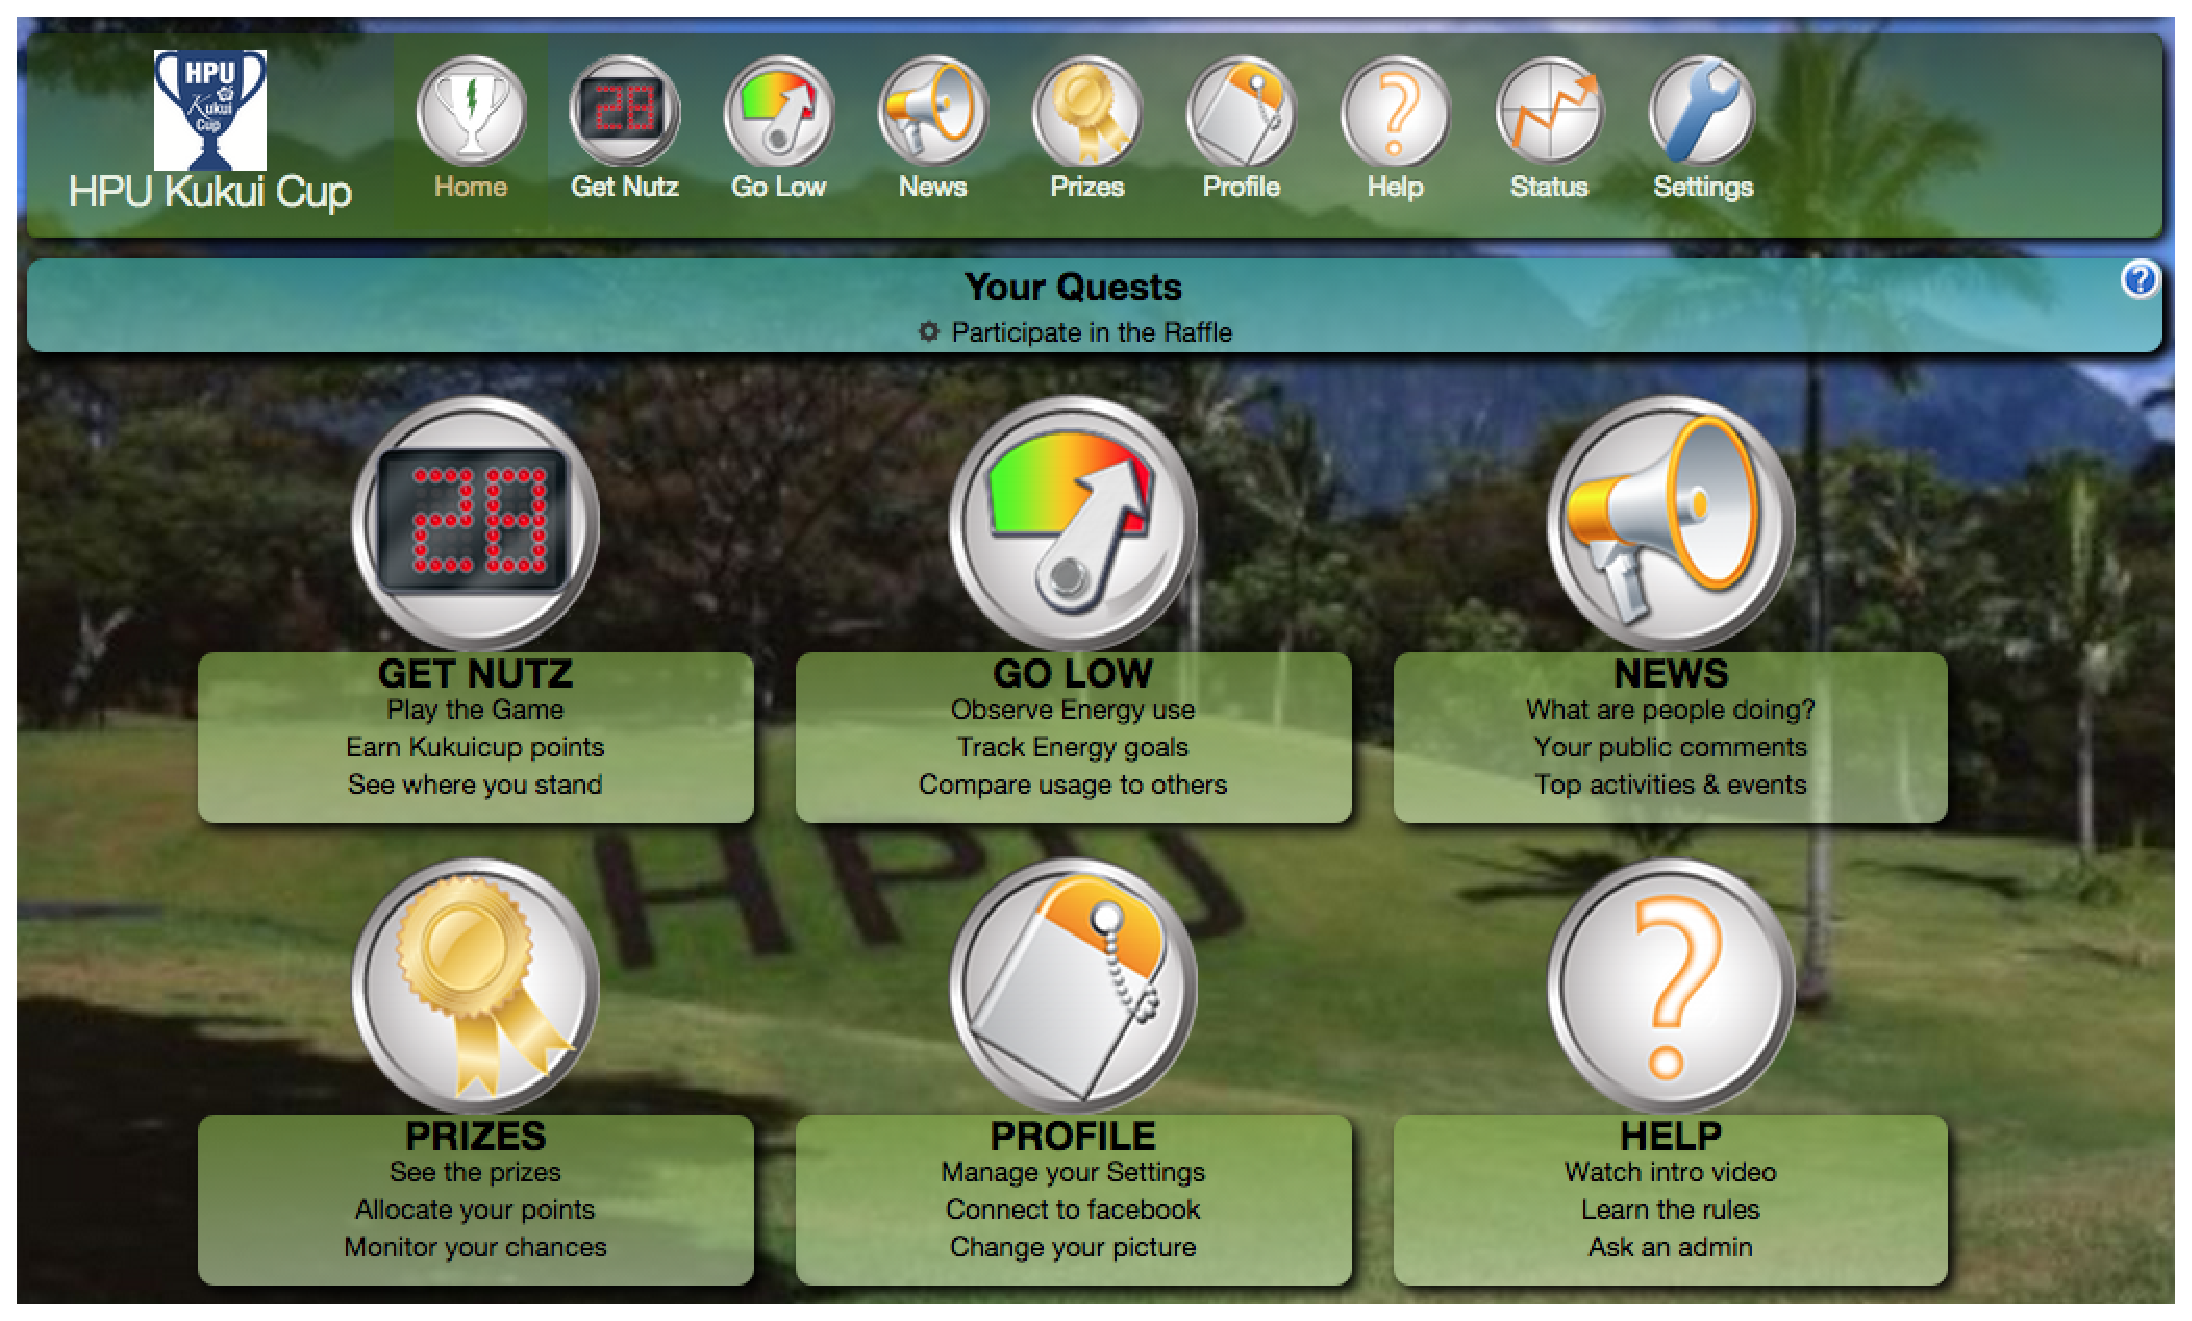
\includegraphics[width=20em]{hpu-homepage}
   \caption{HPU Kukui Cup Challenge Home Page}
   \label{fig:hpu-homepage}
\end{figure}

\subsection{East-West Center}

The EWC Kukui Cup Energy and Water challenge was implemented by an international organization called the East-West Center (EWC) using the Makahiki framework. It was held in 2013 for approximately 600 international students living in their residence halls in Hawaii. The challenge lasts for 2 weeks and includes energy and water saving competition between two residence halls. The residence halls did not have internet-enabled smart meters.

\begin{figure}[ht!]
   \centering
   \includegraphics[width=20em]{ewc-homepage}
   \caption{EWC Kukui Cup Challenge Home Page}
   \label{fig:ewc-homepage}
\end{figure}

\subsection{Holy Nativity School}

A pilot instance of Kukui Cup challenge implemented by using the Makahiki framework was held at the Holy Nativity School (HNS), a private elementary school in Hawaii, in 2013. The pilot instance was organized by the school with the partnership with Project Learning Tree (PLT) GreenSchool! program\cite{plt-greenschools}. The nationwide environmental service-learning program helps improve students’ academic performance in STEM subjects by engaging students in STEM as they solve environmental issues at their school.

\begin{figure}[ht!]
   \centering
   \includegraphics[width=20em]{hns-homepage}
   \caption{HNS Kukui Cup Challenge Home Page}
   \label{fig:hns-homepage}
\end{figure}

\subsection{Customization of the Makahiki Instances}

The following sections describe the different customizations that were done to the above Makahiki instances according to the different organizations' needs.

\subsubsection{Configuration Customization}
The challenge configuration includes the duration of the challenge, the participant accounts, resource such as energy and water settings, learning action configurations, prize and other game mechanics settings. 

Table \autoref{table:challenge-configurations} lists the different configurations between the seven real world instances of Makahiki.

\begin{table}[ht!]
  \centering
  \begin{tabular} {|c|c|c|c|c|c|c|c|c|}
    \hline
    \tabhead{Instances} &
    \tabhead{Participants} &
    \tabhead{Teams} &
    \tabhead{Duration} &
    \tabhead{Rounds} &
    \tabhead{Energy Game} &
    \tabhead{Water Game} &
    \tabhead{Prize Game} &
    \tabhead{Quest Game} \\
    \hline
    UHM2011 & 1000 & 20 & 3 weeks & 3 & Yes & No & Yes & Yes\\
    \hline
    UHM2012 & 1086 & 20 & 9 months & 3 & Yes & No & Yes & Yes\\
    \hline
    UHM2014 & 1093 & 20 & 2 weeks & 3 & Yes & No & Yes & Yes\\
    \hline
    HPU2012 & 190 & 6 & 3 weeks & 3 & Yes & No & Yes & Yes\\
    \hline
    HPU2013 & 190 & 6 & 3 weeks & 3 & Yes & No & Yes & Yes\\
    \hline
    EWC2012 & 130 & 2 & 2 weeks & 3 & Yes  & Yes & No & No\\
    \hline
    HNS2013 & 10 & 2 & 4 weeks & 3 & No & No & Yes & Yes \\
    \hline
  \end{tabular}
  \caption{Challenge Configuration Differences}
  \label{table:challenge-configurations}
\end{table}

As we can see from the Table \autoref{table:challenge-configurations}, the Makahiki framework can be customized to support different size of the team competition with different duration, with energy, water and both competition, as well as the different education contents of
the sponsoring organizations. For example, while UHM and HPU
challenges involved only energy consumption data, the EWC challenge involved both energy
and water consumption data. 

\subsubsection{Content Customization}
Because the different organizations have different sustainability educational needs, they used the Makahiki framework to customize the content, which is shown to student players via the SmartGrid Game mechanics. They can re-use or modify the existing contents came with the Makahiki framework or create new content to be included in the system. The table \autoref{table:sgg-configuration} shows the difference in the type and layout of the educational contents. UHM had the most number of the learning actions while HNS has the least. 

\begin{table}[ht!]
  \centering
  \begin{tabular} {|c|c|c|c|c|c|c|}
    \hline
    \tabhead{Instances} &
    \tabhead{Levels} &
    \tabhead{Activities} &
    \tabhead{Commitments} &
    \tabhead{Events} & 
    \tabhead{Total Actions}\\
    \hline
    UHM2011 & 1 & 40 & 1 & 40  & 499\\
    \hline
    UHM2012 & 7 & 60 & 1 & 40  & 499 \\
    \hline
    UHM2014 & 4 & 34 & 1 & 40  & 499\\
    \hline
    HPU2012 & 3 & 22 & 1 & 40  & 499 \\
    \hline
    HPU2013 & 3 & 33 & 1 & 40  & 499 \\
    \hline
    EWC2012 & 4 & 11 & 1 & 40  & 499 \\
    \hline
    HNS2013 & 2 & 22 & 1 & 40  & 499 \\
    \hline
  \end{tabular}
  \caption{Content Differences}
  \label{table:sgg-configurations}
\end{table}

The layout of the educational content represented in the SmartGrid game is also highly customizable to include different levels, rows and columns. The figures  \autoref{fig:UH-SGG}, \autoref{fig:HPU-SGG}, \autoref{fig:EWC-SGG}, \autoref{fig:GS-SGG} illustrate the content and layout of the educational SmartGrid game in the different Makahiki instances. 

\begin{figure}[http]
	\centering
		\subfigure[UHM 2011 Kukui Cup SmartGrid Game]{\label{fig:uh-2011}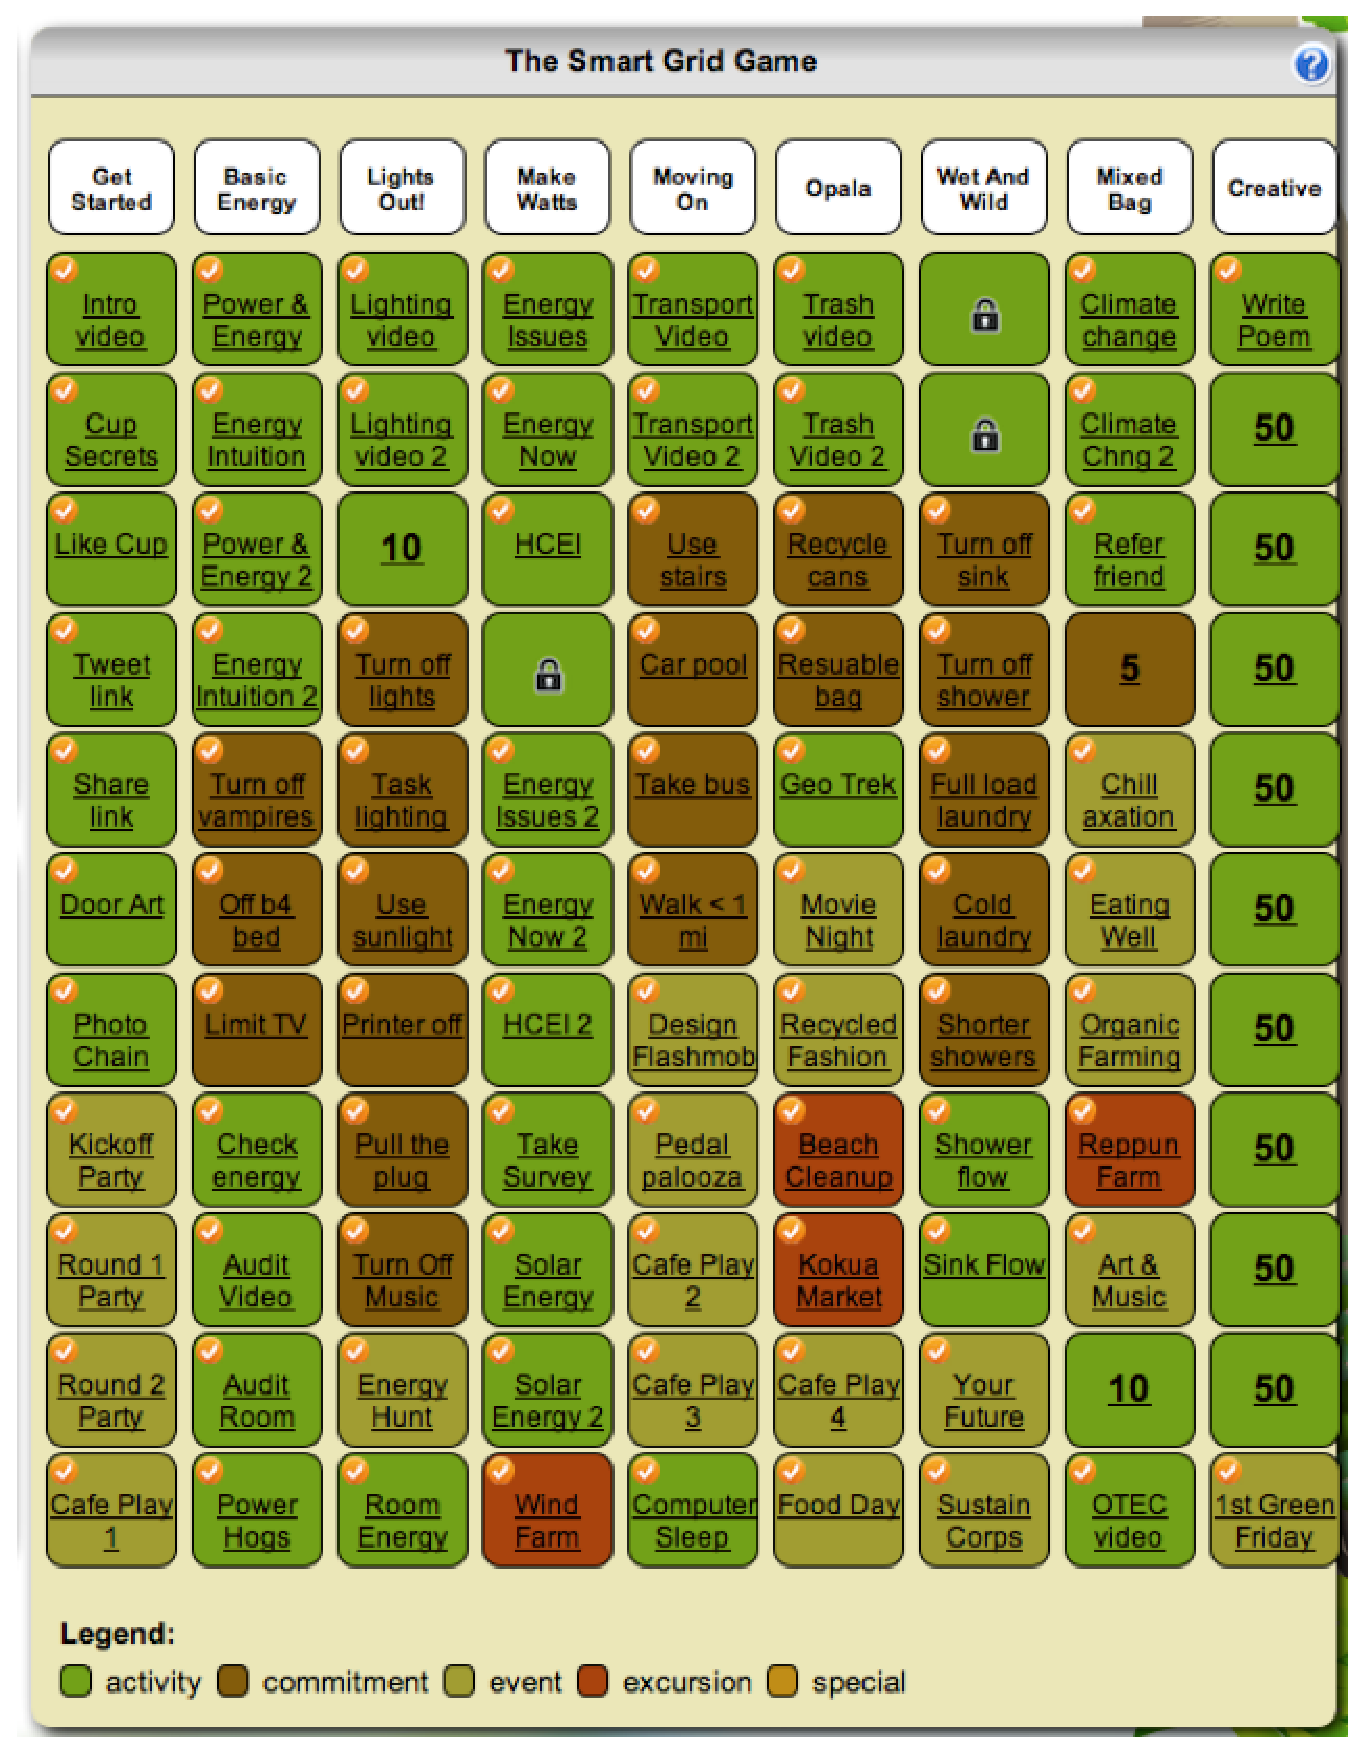
\includegraphics[height=4in,width=3.5in]{UH-SGG-2011.eps}}
		\subfigure[UHM 2012 Kukui Cup SmartGrid Game]{\label{fig:uh-2012}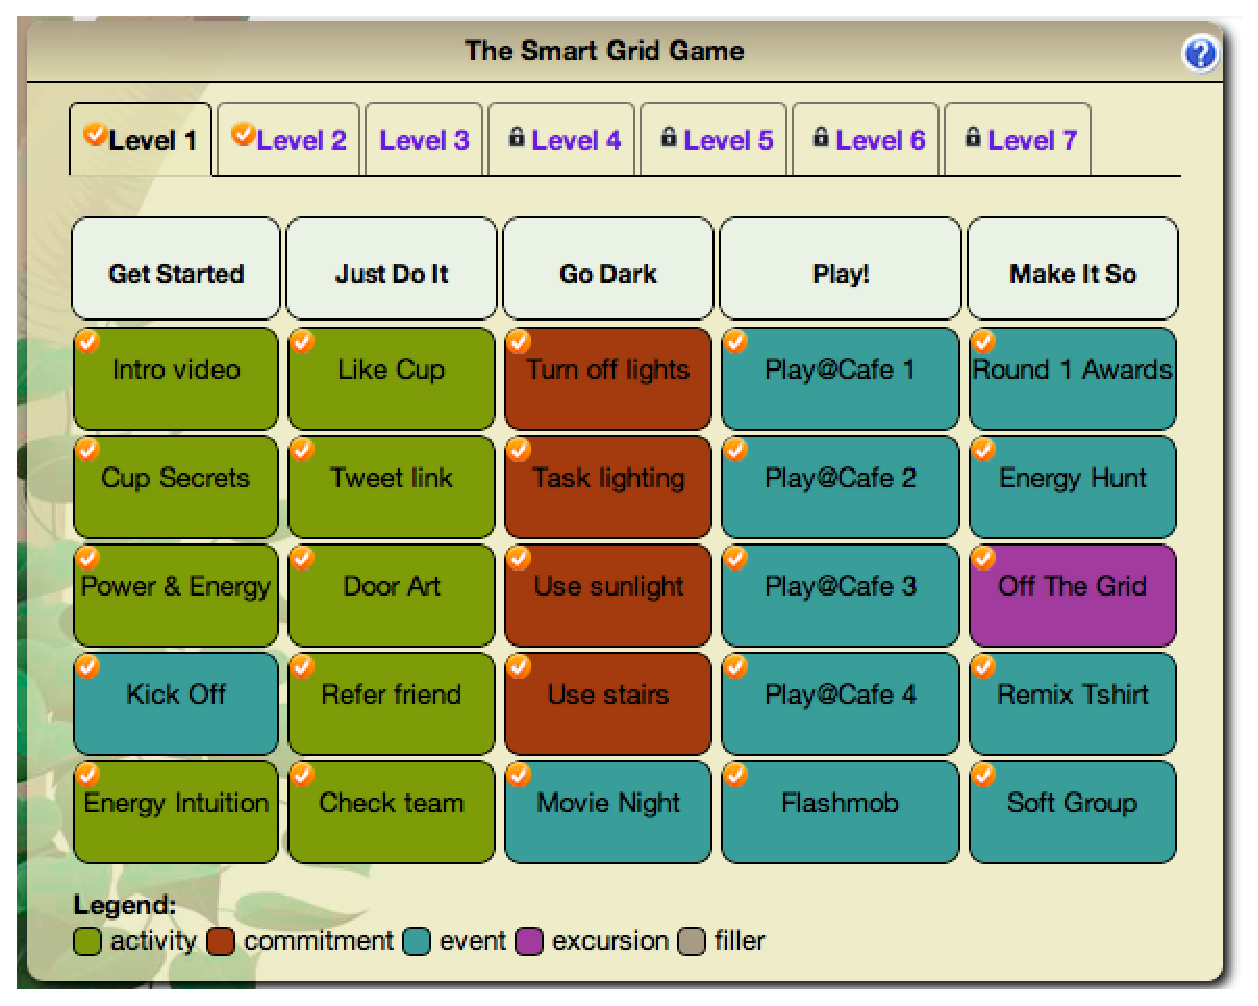
\includegraphics[height=2.3in,width=3.5in]{UH-SGG-2012.eps}}
		\subfigure[UHM 2014 Kukui Cup SmartGrid Game]{\label{fig:uh-2014}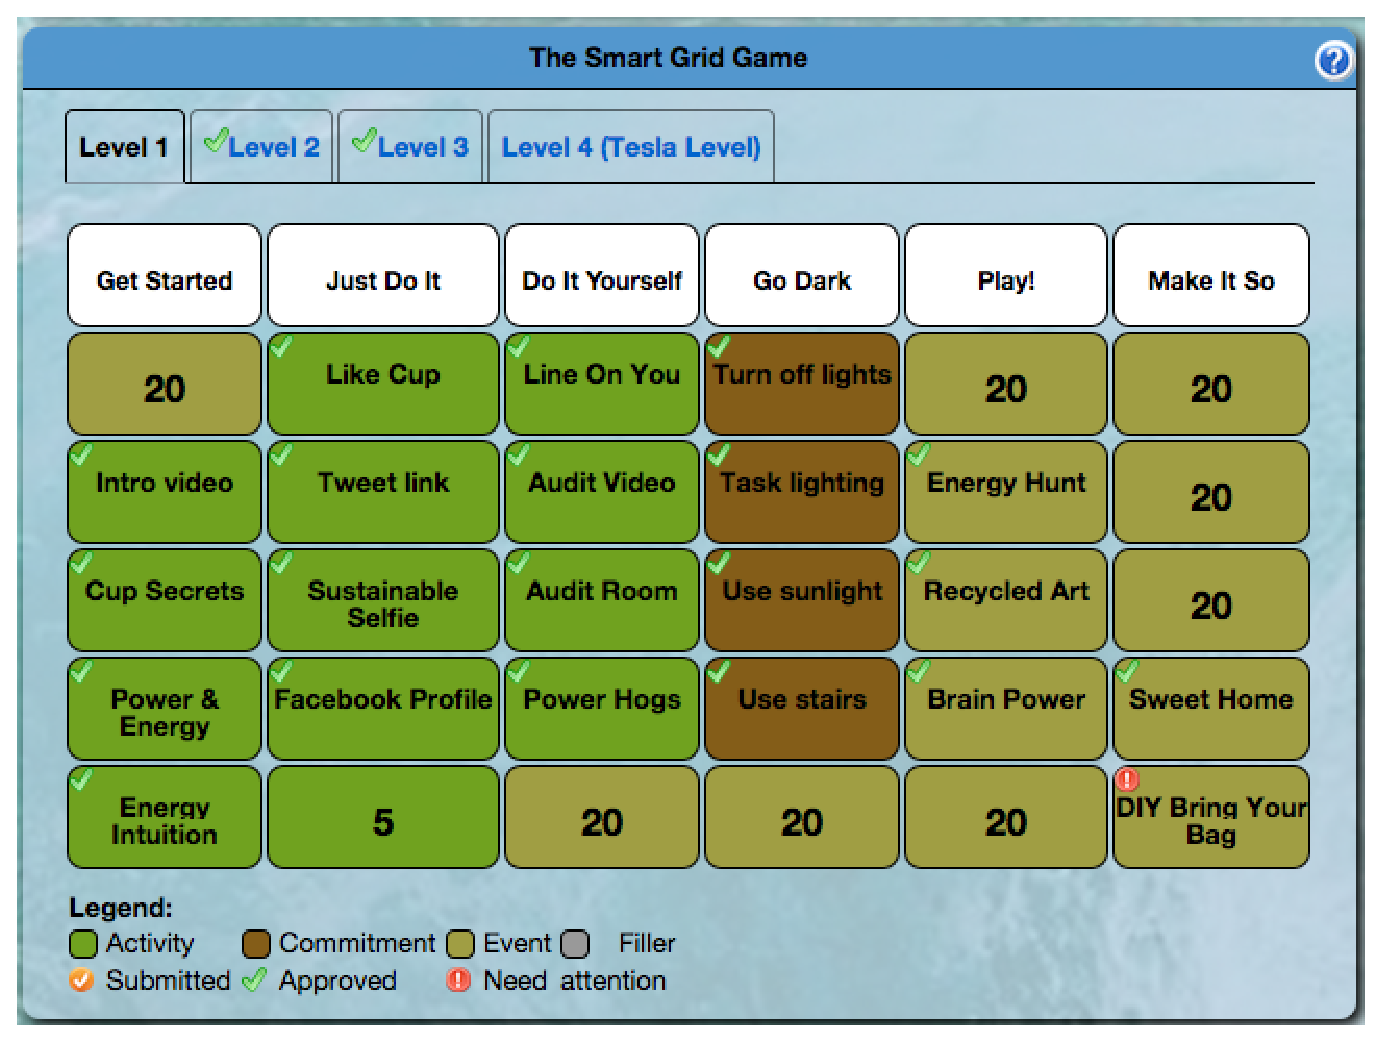
\includegraphics[height=2.3in,width=3.5in]{UH-SGG-2014.eps}}
		\caption{UHM SmartGrid Game Layouts}
		\label{fig:UHM-SGG}
\end{figure}

\begin{figure}[htbp]
	\centering
		\subfigure[HPU SmartGrid Game Level1]{\label{fig:hpu-level1}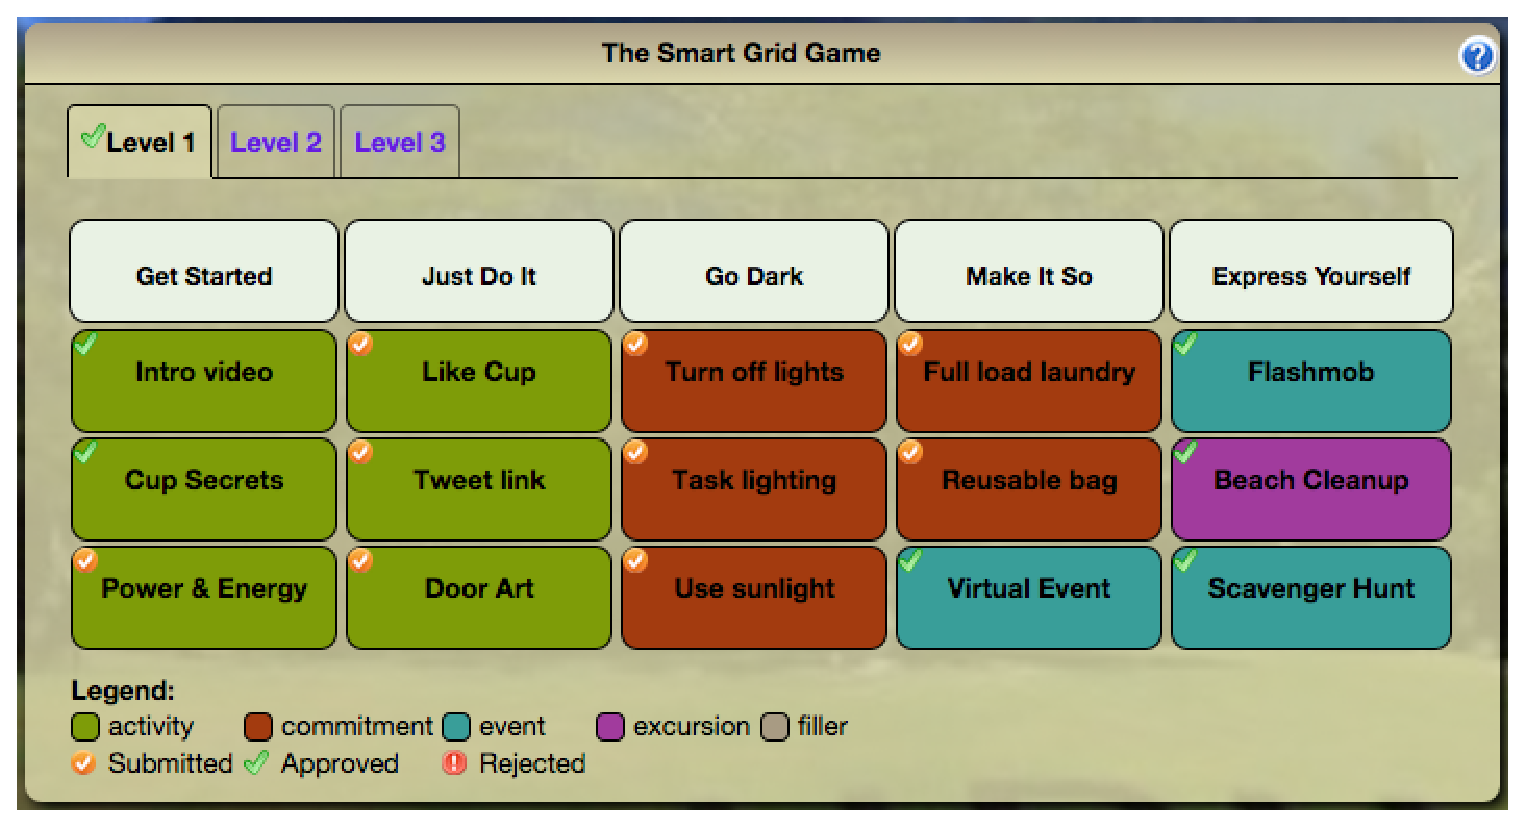
\includegraphics[height=2in,width=3.5in]{HPU-SGG-level1.eps}}
		\subfigure[HPU SmartGrid Game Level2]{\label{fig:hpu-level2}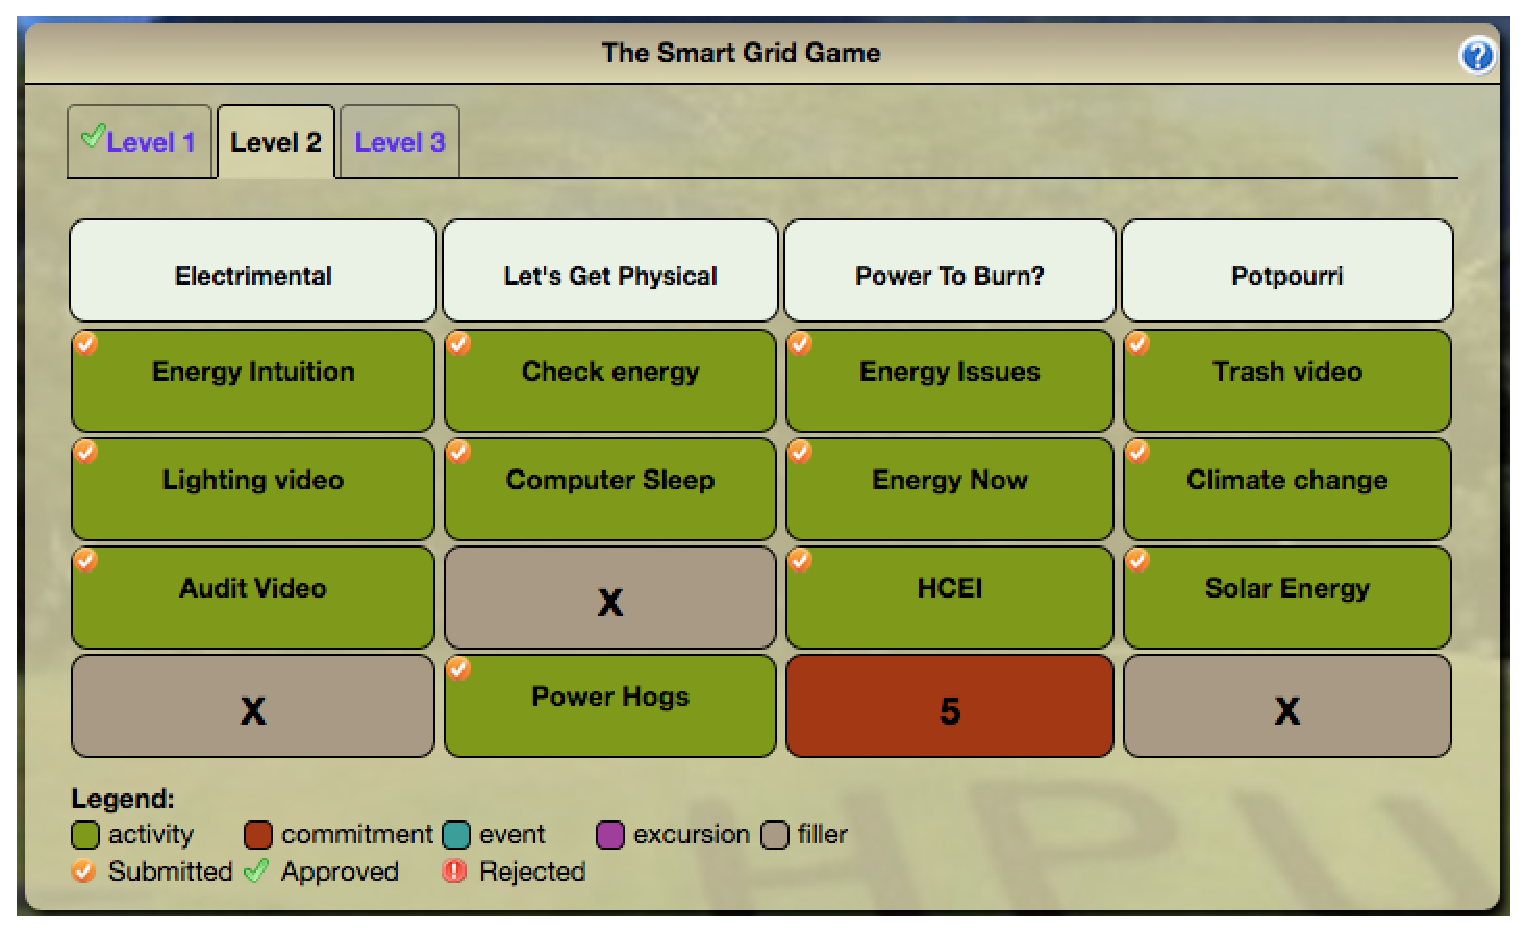
\includegraphics[height=2in,width=3.5in]{HPU-SGG-level2.eps}}
		\subfigure[HPU SmartGrid Game Level3]{\label{fig:hpu-level3}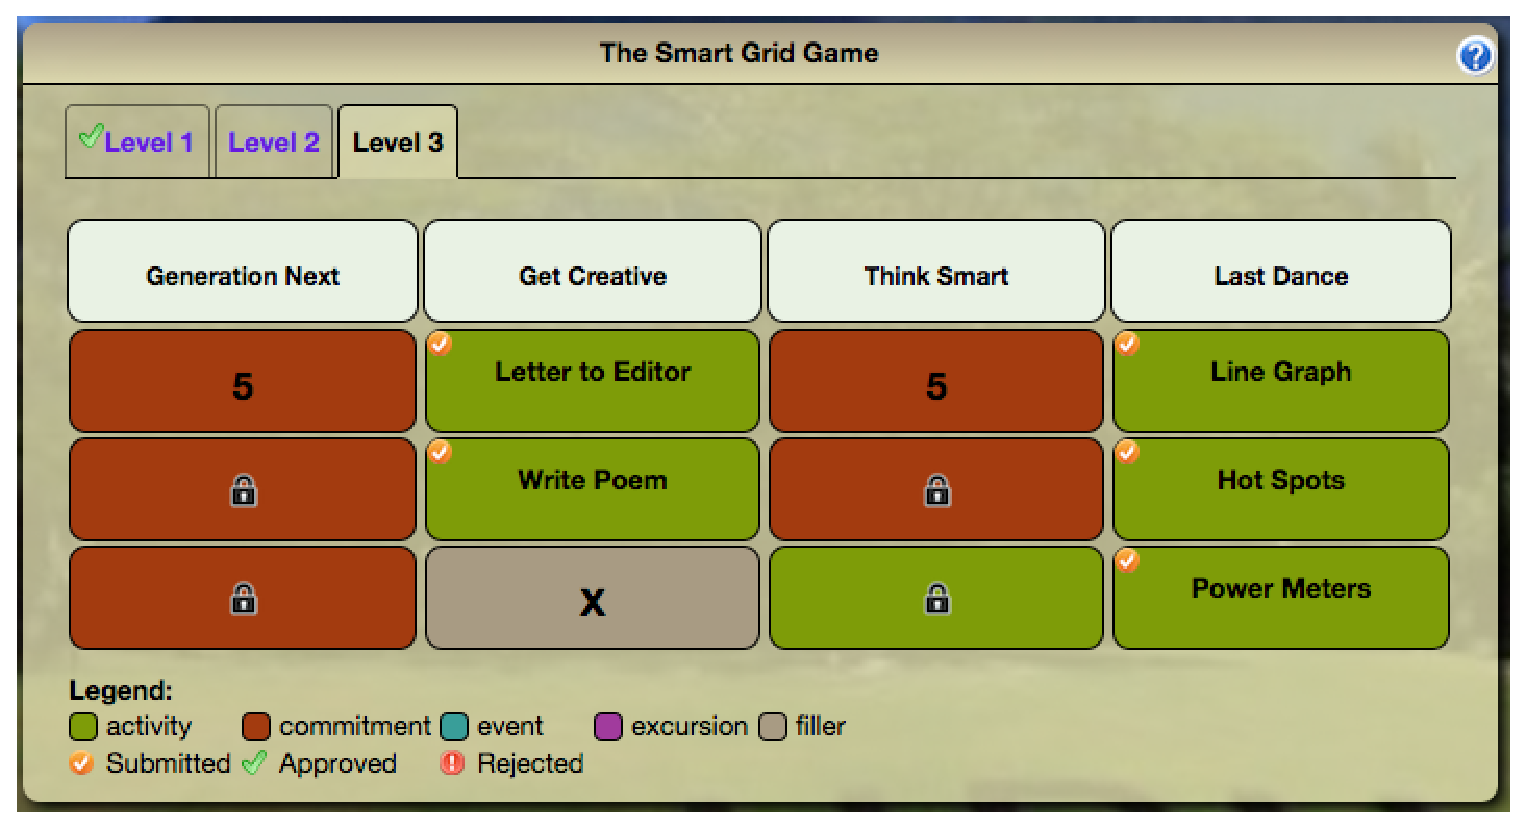
\includegraphics[height=2in,width=3.5in]{HPU-SGG-level3.eps}}
		\caption{HPU SmartGrid Game Layouts}
		\label{fig:HPU-SGG}
\end{figure}

\begin{figure}[htbp]
	\centering
		\subfigure[EWC SmartGrid Game Level1]{\label{fig:ewc-level1}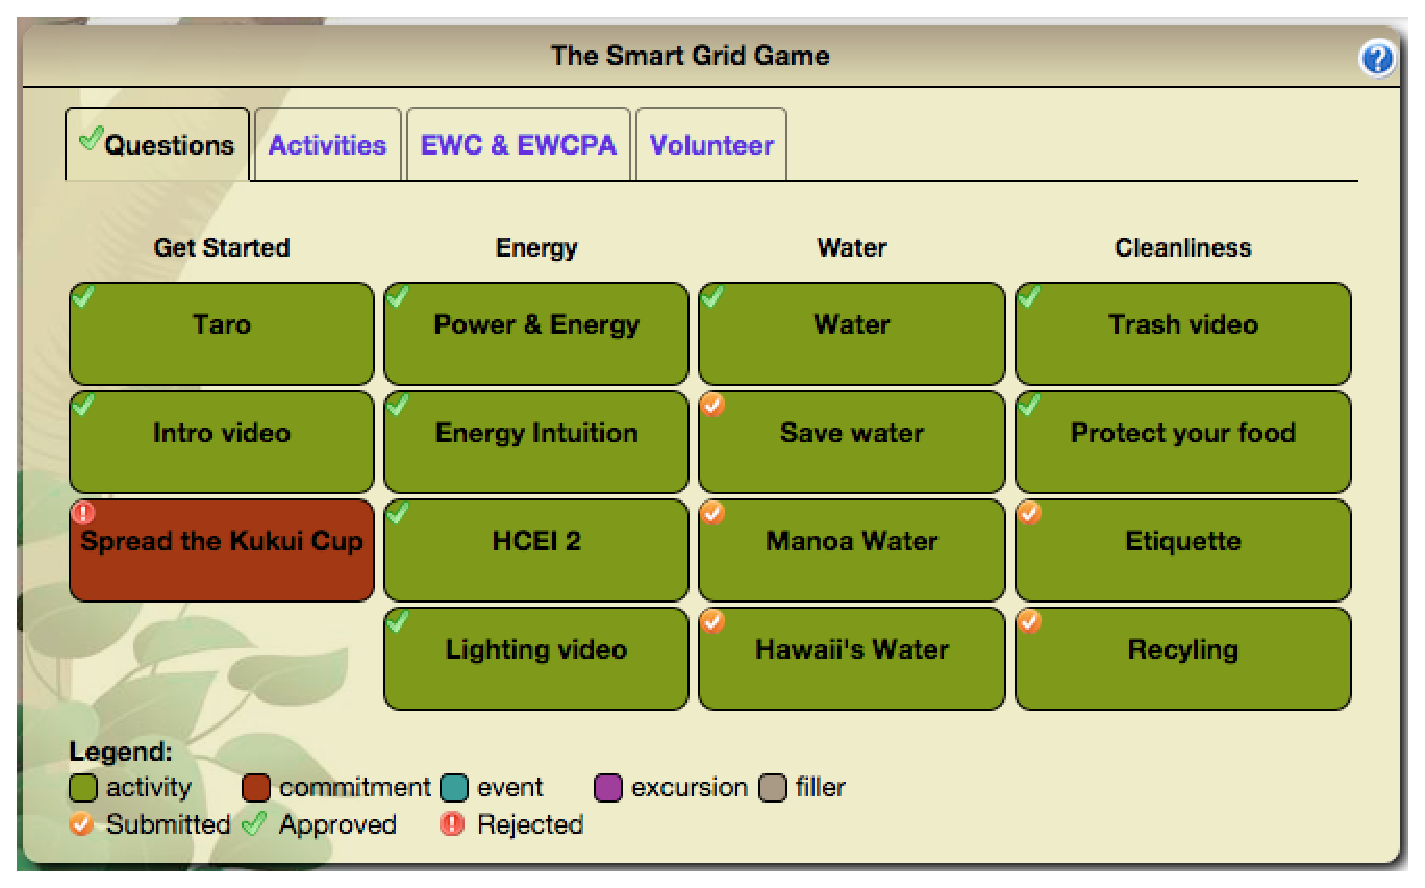
\includegraphics[height=2in,width=3.5in]{EWC-SGG-level1.eps}}
		\subfigure[EWC SmartGrid Game Level2]{\label{fig:ewc-level2}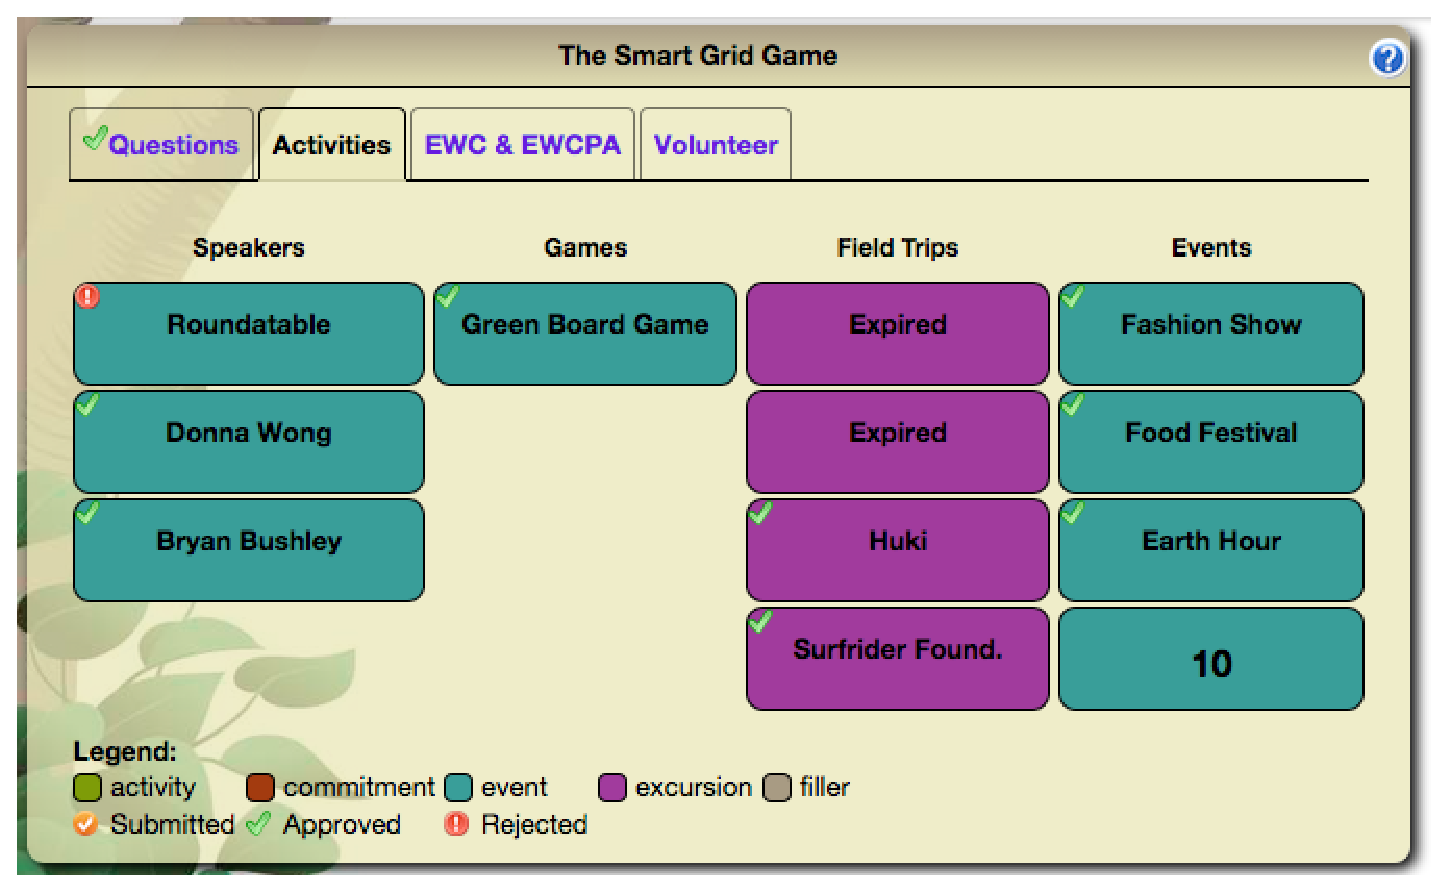
\includegraphics[height=2in,width=3.5in]{EWC-SGG-level2.eps}}
		\subfigure[EWC SmartGrid Game Level3]{\label{fig:ewc-level3}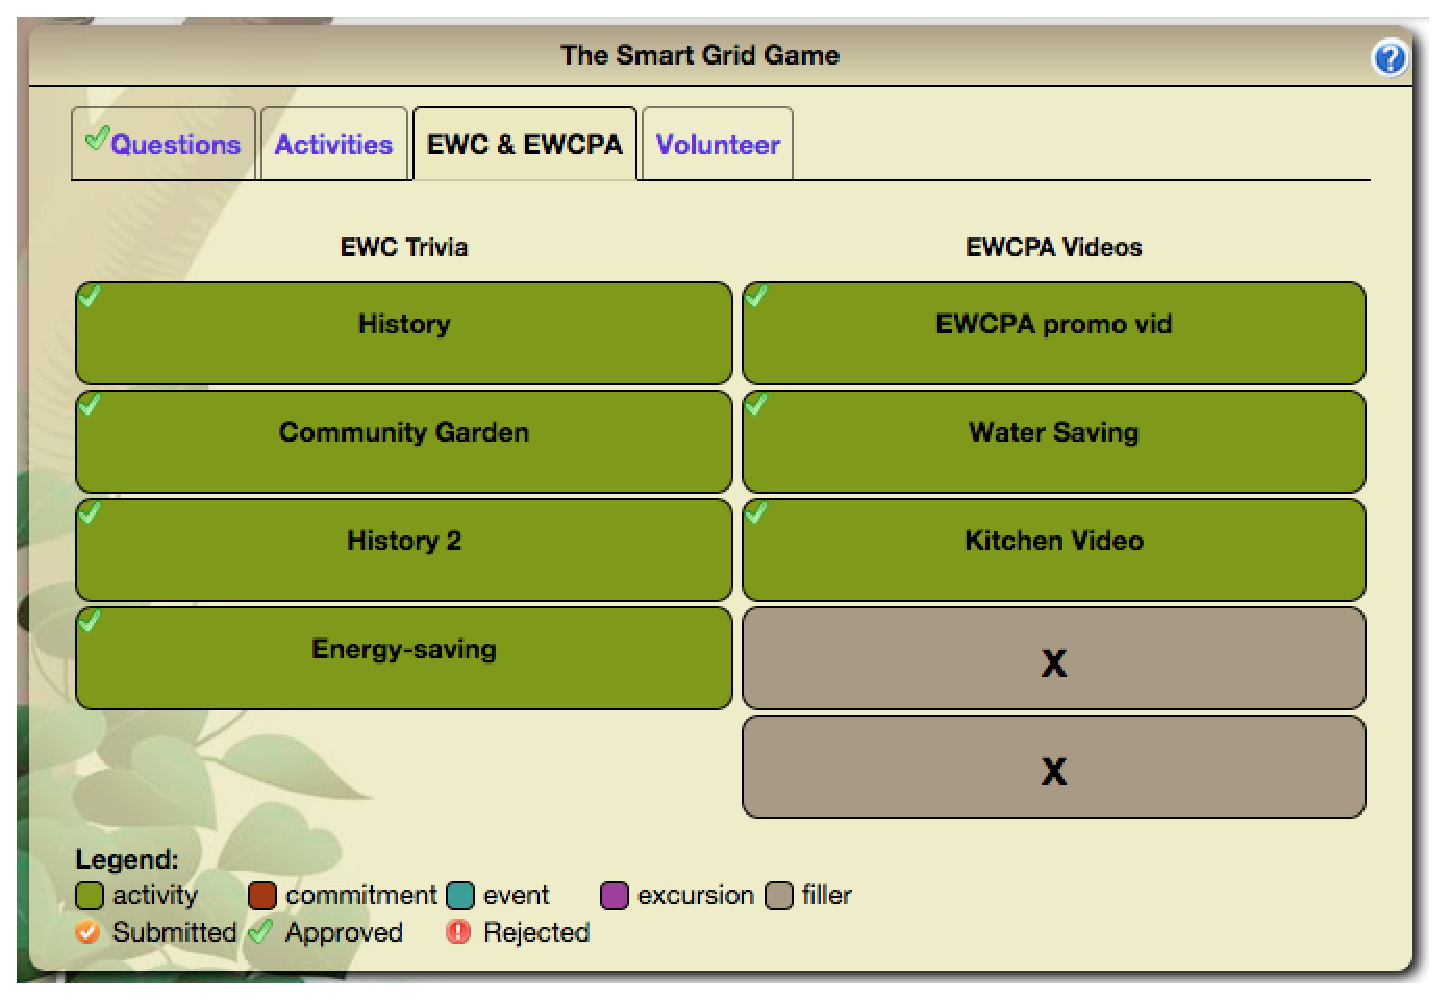
\includegraphics[height=2in,width=3.5in]{EWC-SGG-level3.eps}}
		\subfigure[EWC SmartGrid Game Level4]{\label{fig:ewc-level4}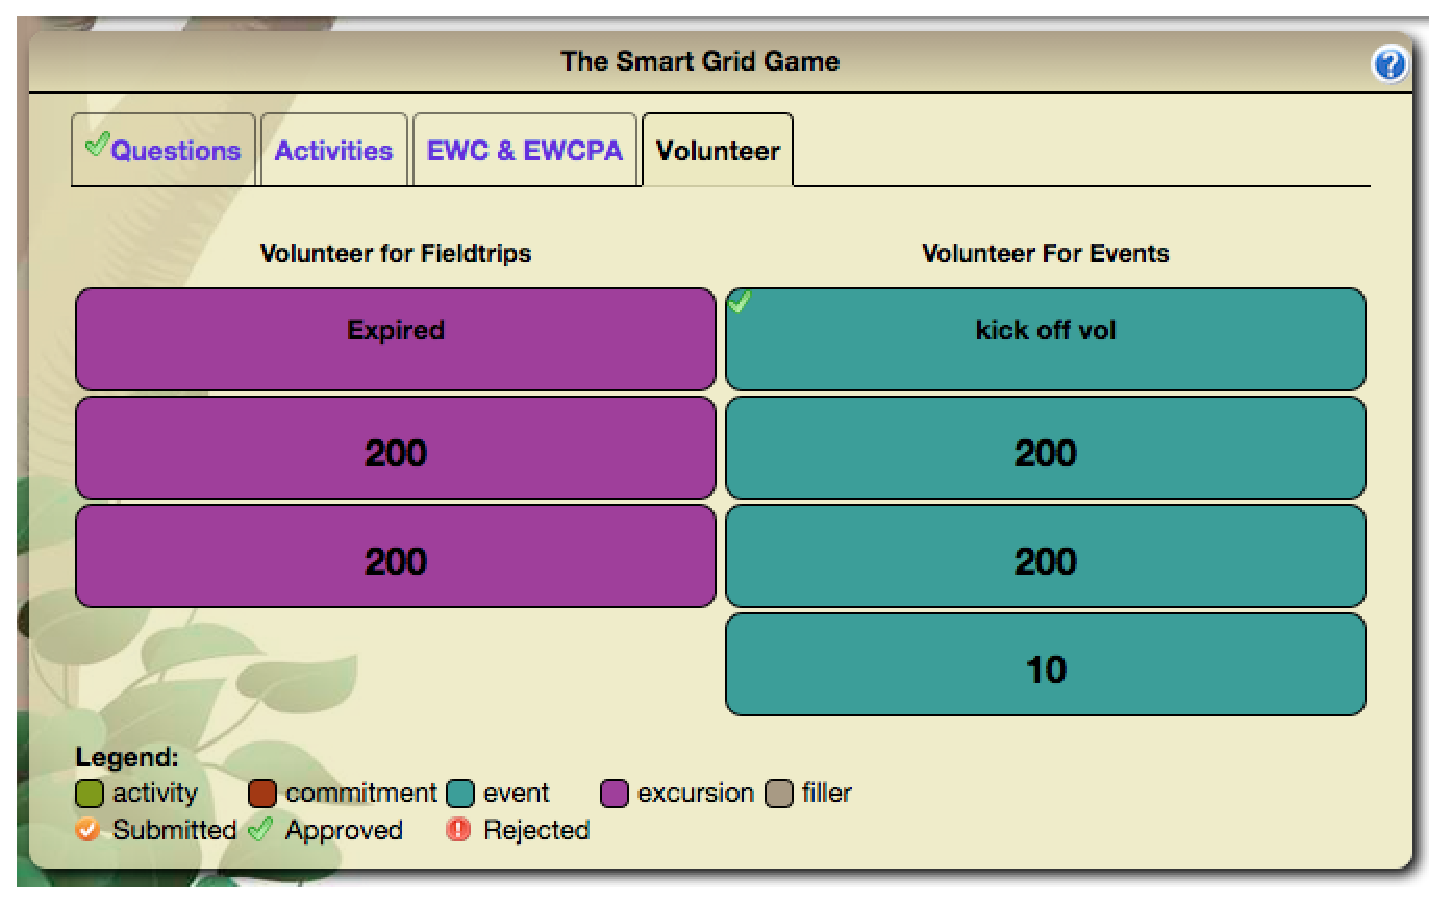
\includegraphics[height=2in,width=3.5in]{EWC-SGG-level4.eps}}
		\caption{EWC SmartGrid Game Layouts}
		\label{fig:EWC-SGG}
\end{figure}

\begin{figure}[htbp]
	\centering
		\subfigure[HNS SmartGrid Game Level1]{\label{fig:gs-level1}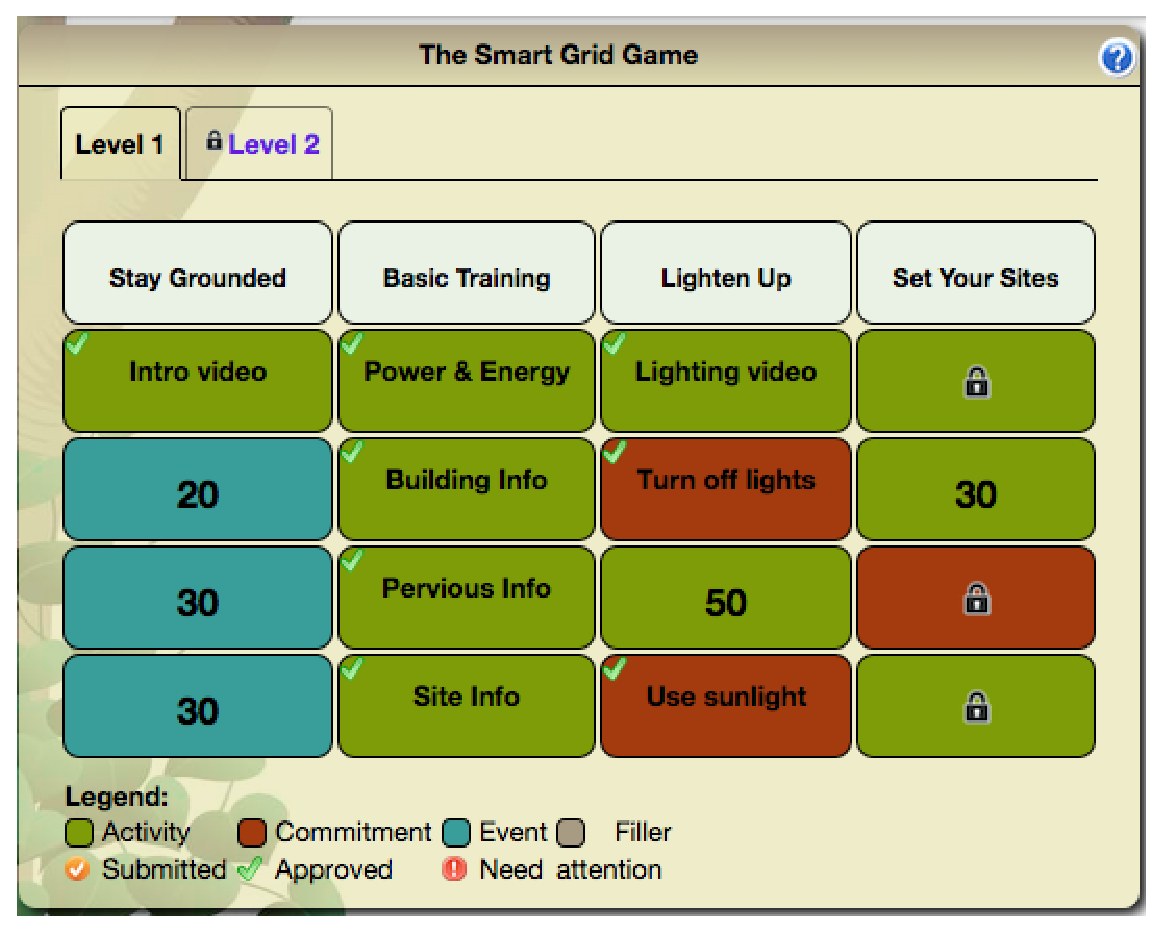
\includegraphics[height=2in,width=3.5in]{GS-SGG-level1.eps}}
		\subfigure[HNS SmartGrid Game Level2]{\label{fig:gs-level2}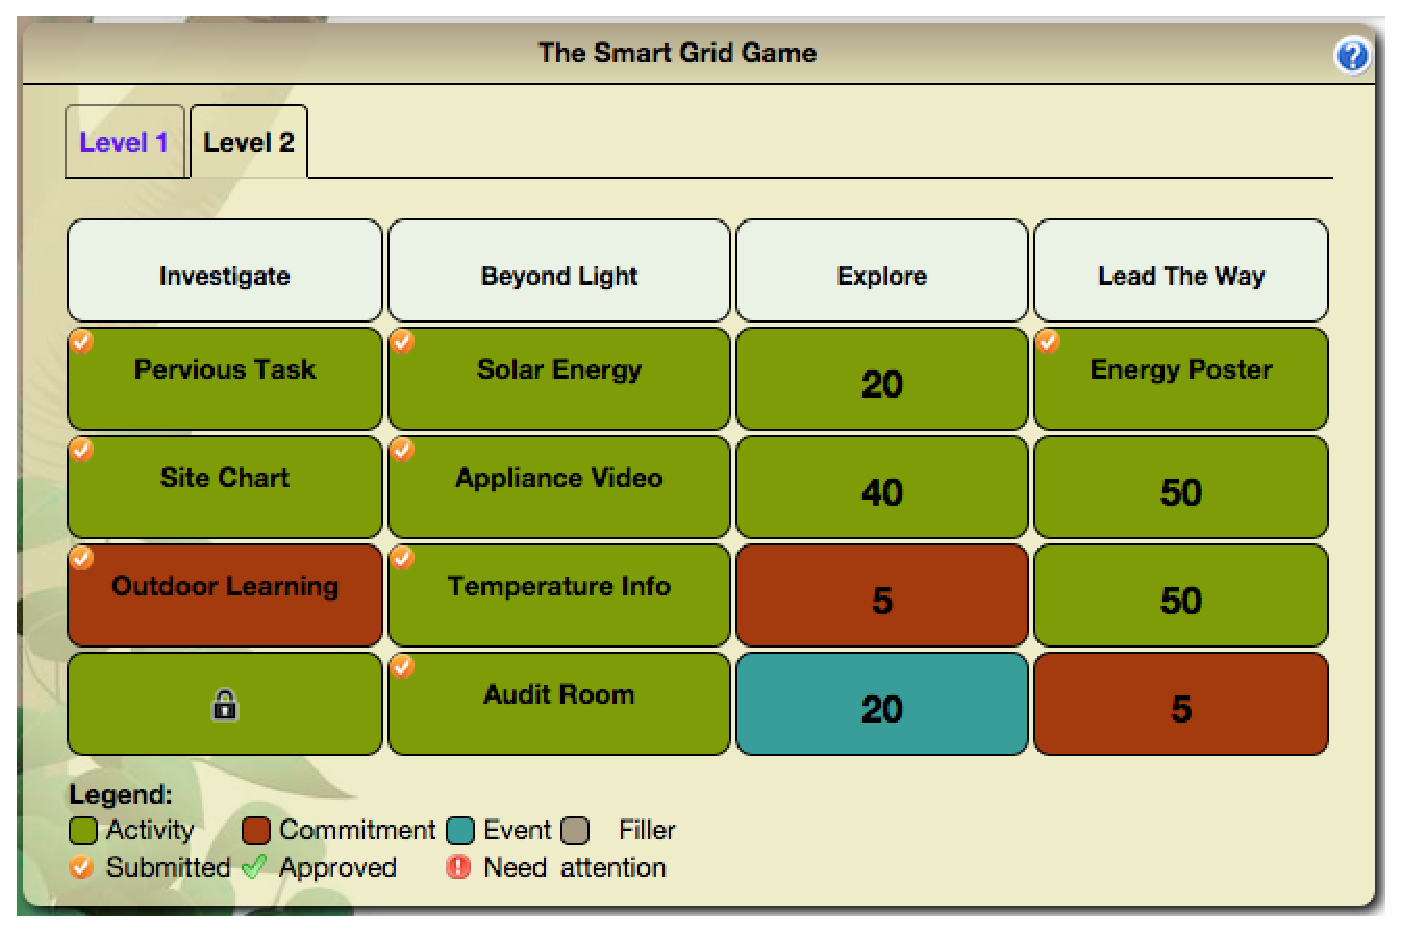
\includegraphics[height=2in,width=3.5in]{GS-SGG-level2.eps}}
		\caption{HNS SmartGrid Game Layouts}
		\label{fig:GS-SGG}
\end{figure}

\subsubsection{Branding Customization}
The look and feel of the challenges website are difference between the different organizations, which is customized using the customization feature of the Makahiki framework. The user interface was customized to ``brand'' each challenge. The list of customizable branding are:

\begin{itemize}
\item logo
\item size name
\item challenge name
\item team label
\item landing page text
\item about page text
\item sponsor text and logo
\item theme
\end{itemize}

\subsubsection{System Configuration}

The system configuration includes the infrastructure hosting, user authentication, and smart meter connections. 

Table \autoref{table:system-configurations} lists the different configurations between the seven real world instances of Makahiki.

\begin{table}[ht!]
  \centering
  \begin{tabular} {|c|c|c|c|c|c|c|}
    \hline
    \tabhead{Instances} &
    \tabhead{Hosting} &
    \tabhead{Authentication} &
    \tabhead{Smart meters} \\
    \hline
    UHM2011 & Local & CAS & Yes \\
    \hline
    UHM2012 & Cloud & CAS & Yes \\
    \hline
    UHM2014 & Cloud & CAS & Yes \\
    \hline
    HPU2012 & Local & LDAP & Yes \\
    \hline
    HPU2013 & Local & LDAP & Yes \\
    \hline
    EWC2012 & Cloud & CAS \& Internal & No \\
    \hline
    HNS2013 & Cloud & Internal & No \\
    \hline
  \end{tabular}
  \caption{System Configuration Differences}
  \label{table:system-configurations}
\end{table}
 
UH and HPU used different metering infrastructure, and EWC collected their resource data manually.  Since the
halls did not have internet-enabled meters, resource consumption data had to be entered by
the game managers manually.

The IT infrastructure at UH and HPU provided
authentication services using CAS (Central Authentication Service) and LDAP, while EWC
used the built-in Django authentication.  

\section{SGSEAM assessment}

The successful creation of serious game challenges by four different organizations
provides evidence that Makahiki can be successfully tailored to the needs of different organizations. This section describes the result of applying a formal assessment method of SGSEAM to the Makahiki framework to assess the strengths and weaknesses of the Makahiki as a serious game framework.

The table \autoref{fig:assessment-overview} provides the overview of applying SGSEAM to Makahiki.

\begin{figure}[ht!]
  \centering
  \begin{tabular}{|c|c|c|}
    \hline
    \multicolumn{1}{|p{0.2\columnwidth}|}{\centering\tabhead{Stakeholder}} &
    \multicolumn{1}{|p{0.5\columnwidth}|}{\centering\tabhead{Assessment Approach}} &
    \multicolumn{1}{|p{0.2\columnwidth}|}{\centering\tabhead{Experiements}}  \\
    \hline
    \multicolumn{1}{|p{0.2\columnwidth}|}{\multirow{4}{*}{Players}} &
    \multicolumn{1}{|p{0.5\columnwidth}|}{Pre Post effectiveness study} &
    \multicolumn{1}{|p{0.2\columnwidth}|}{UHM KC} \\
    \cline{2-3}
    \multicolumn{1}{|p{0.2\columnwidth}|}{} &
    \multicolumn{1}{|p{0.5\columnwidth}|}{Self-reported effectiveness survey} &
    \multicolumn{1}{|p{0.2\columnwidth}|}{UHM KC} \\
    \cline{2-3}    
    \multicolumn{1}{|p{0.2\columnwidth}|}{} &
    \multicolumn{1}{|p{0.5\columnwidth}|}{Self-reported usability survey} &
    \multicolumn{1}{|p{0.2\columnwidth}|}{UHM KC} \\
    \cline{2-3}
    \multicolumn{1}{|p{0.2\columnwidth}|}{} &
    \multicolumn{1}{|p{0.5\columnwidth}|}{Engagement metrics} &
    \multicolumn{1}{|p{0.2\columnwidth}|}{UHM KC} \\
    \hline
    \multicolumn{1}{|p{0.2\columnwidth}|}{\multirow{2}{*}{System admins}} &
    \multicolumn{1}{|p{0.5\columnwidth}|}{In-lab installation study} &
    \multicolumn{1}{|p{0.2\columnwidth}|}{ICS691} \\
    \cline{2-3}
    \multicolumn{1}{|p{0.2\columnwidth}|}{} &
    \multicolumn{1}{|p{0.5\columnwidth}|}{Post-hoc system admin interview} &
    \multicolumn{1}{|p{0.2\columnwidth}|}{HPU KC} \\
    \hline
    \multicolumn{1}{|p{0.2\columnwidth}|}{\multirow{2}{*}{Game designers}} &
    \multicolumn{1}{|p{0.5\columnwidth}|}{In-lab game design study} &
    \multicolumn{1}{|p{0.2\columnwidth}|}{ICS691} \\
    \cline{2-3}
    \multicolumn{1}{|p{0.2\columnwidth}|}{} &
    \multicolumn{1}{|p{0.5\columnwidth}|}{Post-hoc game designer interview} &
    \multicolumn{1}{|p{0.2\columnwidth}|}{HPU KC} \\
    \hline
    \multicolumn{1}{|p{0.2\columnwidth}|}{\multirow{2}{*}{Game managers}} &
    \multicolumn{1}{|p{0.5\columnwidth}|}{In-lab game management study} &
    \multicolumn{1}{|p{0.2\columnwidth}|}{ICS691} \\
    \cline{2-3}
    \multicolumn{1}{|p{0.2\columnwidth}|}{} &
    \multicolumn{1}{|p{0.5\columnwidth}|}{Post-hoc game manager interview} &
    \multicolumn{1}{|p{0.2\columnwidth}|}{HPU KC} \\
    \hline
    \multicolumn{1}{|p{0.2\columnwidth}|}{Developers} &
    \multicolumn{1}{|p{0.5\columnwidth}|}{In-lab game development study} &
    \multicolumn{1}{|p{0.2\columnwidth}|}{ICS691} \\
    \hline
  \end{tabular}
  \caption{SGSEAM assessments for Makahiki}
  \label{fig:assessment-overview}
\end{figure}

\subsection{Makahiki Player Assessment}

We used four approaches to assess the player experience for the Makahiki framework. They are pre-post effectiveness study, self-report effectiveness survey, self-report usability survey, and engagement metrics. The real world Makahiki instances of UHM Kukui Cup challenge were used for the Makahiki player assessments. 

\subsubsection{Pre Post effectiveness study}

In the 2011 Kukui Cup Challenge at the University of Hawaii at Manoa, a serious game implemented using the Makahiki framework, there were over 1000 eligible players for this challenge, who were mostly first
year college students living in the 5 resident halls. The challenge was designed to lasted for 3 weeks and the student players are divided into 20 teams based on the dorm locations where they resided, each team's energy consumption is measured a smart meter installed in the various locations inside the resident hall. Makahiki recorded the energy consumption for the players before, during and after the challenge. Makahiki also recorded detailed logging data from every interaction between the players and the website. 

To assess the effectiveness of the framework for designing games that improve player literacy in sustainability, 
 two energy literacy surveys were conducted, one before the challenge (pre-game) and one after
the challenge (post-game). 24 players completed both surveys. Out of the total 19 energy
literacy questions, the average number of questions answered correctly is 7.54 before the
challenge, and 8.96 after the challenge. This result indicates an 18\% improvement on the
energy literacy.  Non-players as a control condition were also surveyed , and found that
their literacy did not change, indicating that the improvement in player literacy was indeed due to the game.

To assess the effectiveness of the framework for designing games that produce positive change in sustainability
behaviors, The energy consumption data that collected before, during and after the
challenge were used to compare the differences.  Before the challenge, an energy usage baseline was established. 
During the challenge, compared to the baseline, 12 out of the total 20 teams reduced their energy
consumption, with the highest reduction of 16.1\%. However, 3 teams actually increased
their energy consumption, with the highest increase of 11.7\%. Overall, the average
reduction of the 20 teams was very low---approximately 2\%.

\subsubsection{Self-reported effectiveness survey}
A survey to gather the opinions of participants regarding the effect of the challenge to their sustainability behavior was included at the last round of the challenge. 
Two survey questions was used to assess the self-reported perception of the players regarding the interests in energy conservation and sustainability prior and after playing the Kukui Cup. 

In the 2011 UHM Kukui Cup challenge, 43 players completed the survey. The responses to the survey are in free text. We analyzed the free text responses and coded them into three categories: ``Yes'', ``No'', and ``Somewhat''. \autoref{table:interests-in-sustainability} lists results of the responses. \autoref{fig:effect-prior-after} illustrates the percentages of self-reported interests in the sustainability prior to the KuKui Cup and the effect after playing the Kukui Cup.

\begin{table}[ht!]
  \centering
  \begin{tabular} {|p{0.6\linewidth}|c|c|c|}
    \hline
    \tabhead{\multirow{2}{*}{Question}} & \multicolumn{3}{c|}{\tabhead{Number of Responses}} \\
    \cline{2-4}
    \tabhead{} & \tabhead{Yes} & \tabhead{No } & \tabhead{Somewhat}\\
    \hline
    Prior to playing the Kukui Cup, were you interested in energy conservation? & 24 & 8 & 11\\
    \hline
    Has the Kukui Cup increased your interest in energy conservation and sustainability?& 37 & 0 & 6 \\
    \hline
  \end{tabular}
  \caption{Interests in sustainability prior and after the KC (2011 UHM KC, n=43)}
  \label{table:interests-in-sustainability}
\end{table}

\begin{figure}[htbp]
	\centering
		\subfigure[interests in sustainability prior]{\label{fig:effect-prior}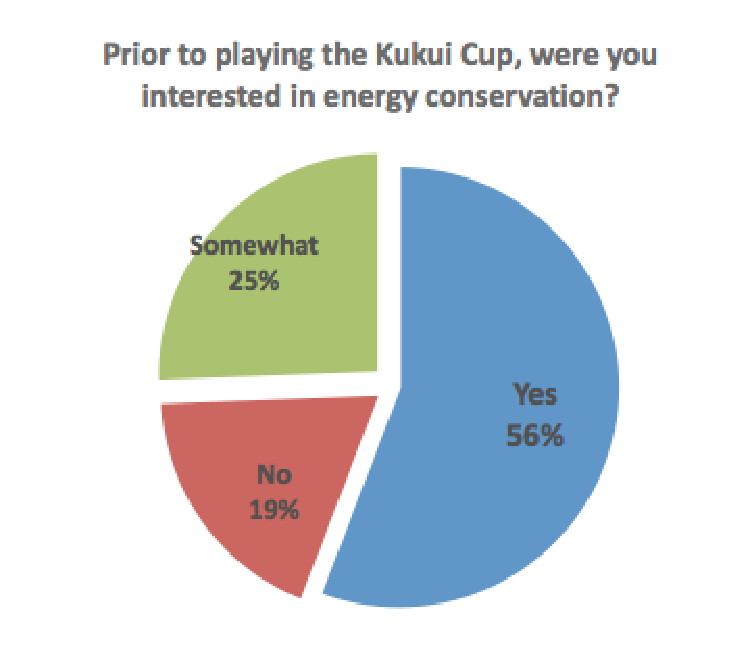
\includegraphics[height=2.2in]{effect-prior.eps}}
		\subfigure[increased interests in sustainability after]{\label{fig:effect-after}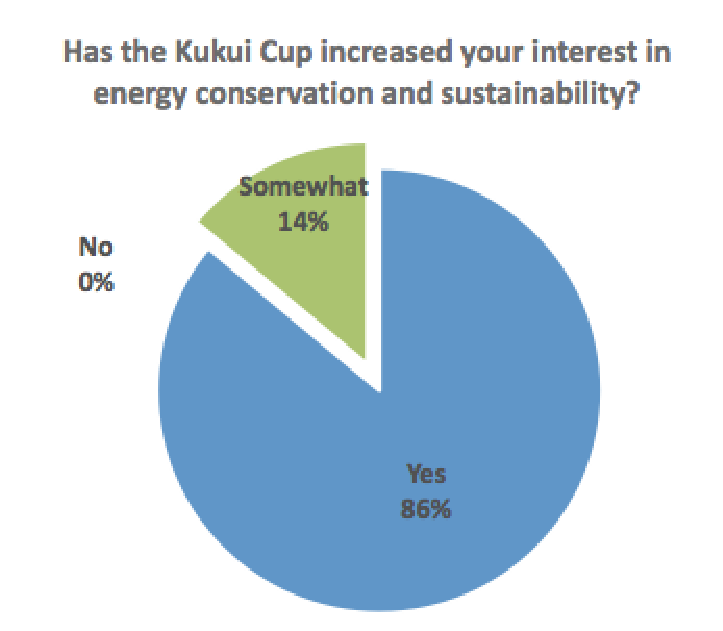
\includegraphics[height=2.2in]{effect-after.eps}}
		\caption{Interests in Sustainability Prior and After the UHM 2011 KC}
		\label{fig:effect-prior-after}
\end{figure}

The self-reported responses indicates that there are a small percentage (19\%) of players were not interested in the sustainability prior to the Kukui Cup. After playing the Kukui Cup, 100\% of responses reported an affirmative or somewhat increase of interests in sustainability. 

In 2012 UHM Kukui Cup challenge, the same survey questions were included the last round. 44 players completed both the two questions. \autoref{table:interests-in-sustainability-2012} lists results of the responses. \autoref{fig:effect-prior-after-2012} illustrates the percentages of self-reported interests.

\begin{table}[ht!]
  \centering
  \begin{tabular} {|p{0.6\linewidth}|c|c|c|}
    \hline
    \tabhead{\multirow{2}{*}{Question}} & \multicolumn{3}{c|}{\tabhead{Number of Responses}} \\
    \cline{2-4}
    \tabhead{} & \tabhead{Yes} & \tabhead{No } & \tabhead{Somewhat}\\
    \hline
    Prior to playing the Kukui Cup, were you interested in energy conservation? & 28 & 4 & 12\\
    \hline
    Has the Kukui Cup increased your interest in energy conservation and sustainability?& 37 & 5 & 2 \\
    \hline
  \end{tabular}
  \caption{Interests in sustainability prior and after the KC (2012 UHM KC, n=44)}
  \label{table:interests-in-sustainability-2012}
\end{table}

\begin{figure}[htbp]
	\centering
		\subfigure[interests in sustainability prior]{\label{fig:effect-prior}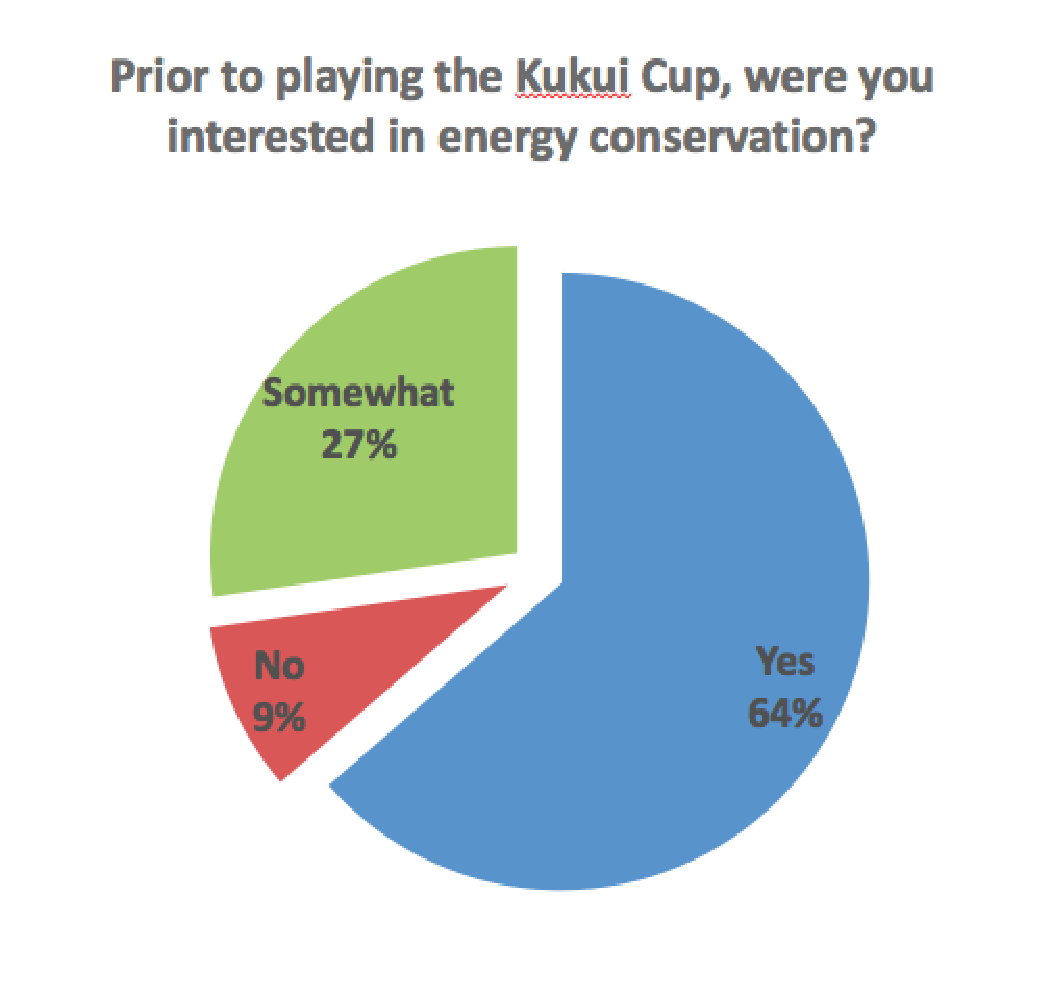
\includegraphics[height=2.2in]{effect-prior-2012.eps}}
		\subfigure[increased interests in sustainability after]{\label{fig:effect-after}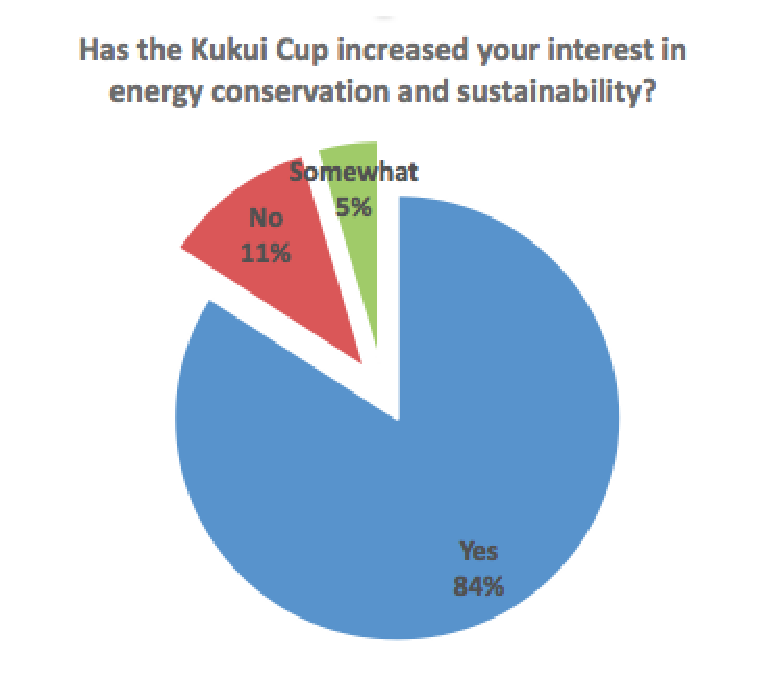
\includegraphics[height=2.2in]{effect-after-2012.eps}}
		\caption{Interests in Sustainability Prior and After the 2012 UHM KC}
		\label{fig:effect-prior-after-2012}
\end{figure}

The self-reported responses from 2012 KC indicates that there are a smaller percentage (9\%) of players than 2011 KC that were not interested in the sustainability prior to the Kukui Cup. After playing the Kukui Cup, 89\% of responses reported an affirmative or somewhat increase of interests in sustainability. There are 5 players (11\%)  reported that there is no changes of interests in sustainability. A closer look at the data indicates that the 5 players that reported no changes of interests also answered ``Yes'' or ``Somewhat'' interested to the sustainability prior to the Kukui Cup. The 4 players that reported no interests in sustainability also reported that playing KC had increased their interests.

The followings are some sample responses from the students who considered the Kukui Cup had increased their interests in sustainability:
 
 \begin{itemize}
 \item Yes. I'm more aware of everything I am using.
\item I've been interested, but the Kukui Cup has expanded and broadened my mind on what else I can be doing to help with conservation and sustainability. I think people are genuinely concerned, they just don't know how to exactly conduct them, or what other ways they can do it.
\item Yes, it made me realize that you can save a lot of money by turning off and unplugging a few things. (Hopefully lower tuition? =D )
\item It has increased my interest since I didn't know much about how much energy were using.
\item Some workshops made me think differently of how I use energy. Makes alternatives more interesting for me.
\item It taught me some new interesting facts about renewable energy and made me more aware.
\end{itemize}

There was a question in the 2011 KC survey tasking about the players' perception about how would they describe the Kukui Cup. The players were asked to check all that applies to their agreement to the following descriptions of the Kukui Cup: Educational, Fun, Addictive, So-so, Difficult, Boring, Not useful, and Other where they will type in their free text response. There were 43 responses from the 2011 KC survey. The number of responses and their percentage are listed in the \autoref{table:how-is-kc}.

\begin{table}[ht!]
  \centering
  \begin{tabular} {|c|c|c|}
    \hline
    \tabhead{Question: How would you describe the Kukui Cup?} & \tabhead{Number of Responses} & \tabhead{Percentage}\\
    \hline
Educational	& 41 & 95\%\\
    \hline
Fun	& 39 & 91\% \\
    \hline
Addictive	 &19 & 44\%\\
    \hline 
So-so	& 9 & 21\%\\
    \hline
difficult	& 3 & 7\%\\
    \hline
Boring	& 1 & 2\%\\
    \hline
not useful	& 0 & 0\\
    \hline
Other & 5 & 12\%\\   
    \hline 
  \end{tabular}
  \caption{Self-reported Perception of the Kukui Cup in 2011 UHM KC (n=43)}
  \label{table:how-is-kc}
\end{table}
	
Majority of the responses indicated the players perceived the Kukui Cup as ``Educational'' (95\%) and ``Fun'' (91\%). There are 44\% players perceived Kukui Cup as ``Addictive". On the other hand, there are 1 player (2\%) considered the Kukui Cup as``Boring". The ``Other'' responses are: ``AWSOME-NESS''(1), ``engaging''(1), ``fun competition''(1), ``Great way to bond with others''(1), ``impressive''(1).

A survey question was also asked about the players' self reported behavior change during the challenge in the 2012 UHM Kukui Cup. The question is ``Did you change your behavior during the competition based on the commitment(s) you made? if so, how?". It is a free response question. 45 players completed the survey in the 2012 UHM KC. I categorized the free text responses into three categories: ``Yes'', `already a habit'', and ``no''. The results are listed in \autoref{table:behavior-change}.

\begin{table}[ht!]
  \centering
  \begin{tabular} {|p{0.5\linewidth}|c|c|}
    \hline
    \tabhead{Question: Did you change your behavior during the competition based on the commitment(s) you made?} & \tabhead{Number of Responses} & \tabhead{Percentage}\\
    \hline
Yes	& 39 & 87\%\\
    \hline
Already a habit	& 4 & 9\% \\
    \hline
No	 &2 & 4\%\\
    \hline 
  \end{tabular}
  \caption{Self-reported Behavior Changes in 2012 UHM KC (n=45)}
  \label{table:behavior-change}
\end{table}

The examples of a ``Yes'' response are:
\begin{itemize}
\item ``I changed my behavior during the commitments but found myself doing the same things i did before after they were over.''
\item ``Yes, because knowing the facts of how much energy we use has helped me realize that I have been wasting money and energy.''
\item ``yes, my behavior has changed during the competition. I'm more aware of the things i do such as turning off appliances when not in use, as well as using more natural energy such as sunlight, rather than electricity.''
\end{itemize}

A ``Already a habit'' response is that the commitments already become part of the daily habit. The examples are:
\begin{itemize}
\item ``Most of the commitments I made I already did.''
\item ``I always turn off my lights when I leave the room, use cold water to wash my clothes, and I lessen my meat intake. ''
\end{itemize}

The self-reported survey results indicate in general, the players of Makahiki considered their experiences are positive and there had some self-reported impacts to their sustainability behaviors. 

\subsubsection{Self-reported usability survey}

A survey to gather the opinions of players regarding the usability of the website was added during the last round of the challenge. 

The players were asked to rate how much you agree with the following 4 usability statements in a likert scale (Strongly disagree, Disagree, Neutral, Agree, Strongly agree):
\begin{enumerate}
\item ``It was easy to find what I was looking for in the website.''
\item ``The website was responsive. I did not wait too long after I clicked on something.''
\item ``The website provided adequate help in teaching me how to play the game.''
\item ``I understood the rules of the game and how to play.''
\end{enumerate}

The questions were asked in both the 2011 and 2014 Kukui Cup in the University of Hawaii at Manoa, 43 players completed the survey in the 2011 KC while 18 players completed in the 2014 KC.  

\autoref{table:self-report-usability-2011}  and \autoref{table:self-report-usability-2014}  lists the results of the self-reported usability responses for both 2011 and 2014 Kukui Cup at UHM.

\begin{table}[ht!]
  \centering
  \begin{tabular} {|p{0.45\linewidth}|p{0.09\linewidth}|p{0.08\linewidth}|p{0.08\linewidth}|p{0.08\linewidth}|p{0.08\linewidth}|}
    \hline
    \tabhead{} & \tabhead{Strongly disagree} & \tabhead{Disagree} & \tabhead{Neutral} & \tabhead{Agree} & \tabhead{Strongly agree}\\
    \hline
It was easy to find what I was looking for in the website.& 2 & 1 & 2 & 14 & 24 \\
    \hline
The website was responsive. I did not wait too long after I clicked on something.& 2 & 1 & 1& 19 & 20 \\
    \hline
The website provided adequate help in teaching me how to play the game.	 & 1 & 1 & 1 & 16 & 24\\
    \hline
I understood the rules of the game and how to play	& 1& 1 & 0 & 12 & 29\\
    \hline 
  \end{tabular}
  \caption{Self-reported Usability in 2011 UHM KC (n=43)}
  \label{table:self-report-usability-2011}
\end{table}

\begin{table}[ht!]
  \centering
  \begin{tabular} {|p{0.45\linewidth}|p{0.09\linewidth}|p{0.08\linewidth}|p{0.08\linewidth}|p{0.08\linewidth}|p{0.08\linewidth}|}
    \hline
    \tabhead{} & \tabhead{Strongly disagree} & \tabhead{Disagree} & \tabhead{Neutral} & \tabhead{Agree} & \tabhead{Strongly agree}\\
    \hline
It was easy to find what I was looking for in the website.& 0 & 0 & 1 & 9 & 8\\
    \hline
The website was responsive. I did not wait too long after I clicked on something.& 0 & 4 & 2 & 10 & 2 \\
    \hline
The website provided adequate help in teaching me how to play the game.& 0 & 0 & 2 & 10 & 6 \\
    \hline
I understood the rules of the game and how to play.& 0 & 0 & 1 & 10 & 7 \\
    \hline 
  \end{tabular}
  \caption{Self-reported Usability in 2014 UHM KC (n=18)}
  \label{table:self-report-usability-2014}
\end{table}

\autoref{fig:self-report-usability-2011-2014} illustrates the self-reported usability measurements in both 2011 KC and 2014 KC. Majority of players reported that they agreed that the usability of the website is good with one exception of responsiveness from the 2014 responses. 4 out of 18 players (22\%) of 2014 KC reported that they considered the website is not very responsive. Comparing to the result of the 2011 KC, this indicates that there may be a perceived performance downgrade in the 2014 KC website.

\begin{figure}[ht!]
	\centering
		\subfigure[2011 Self-reported Usability Measurements(n=43)]{\label{fig:self-report-usability-2011}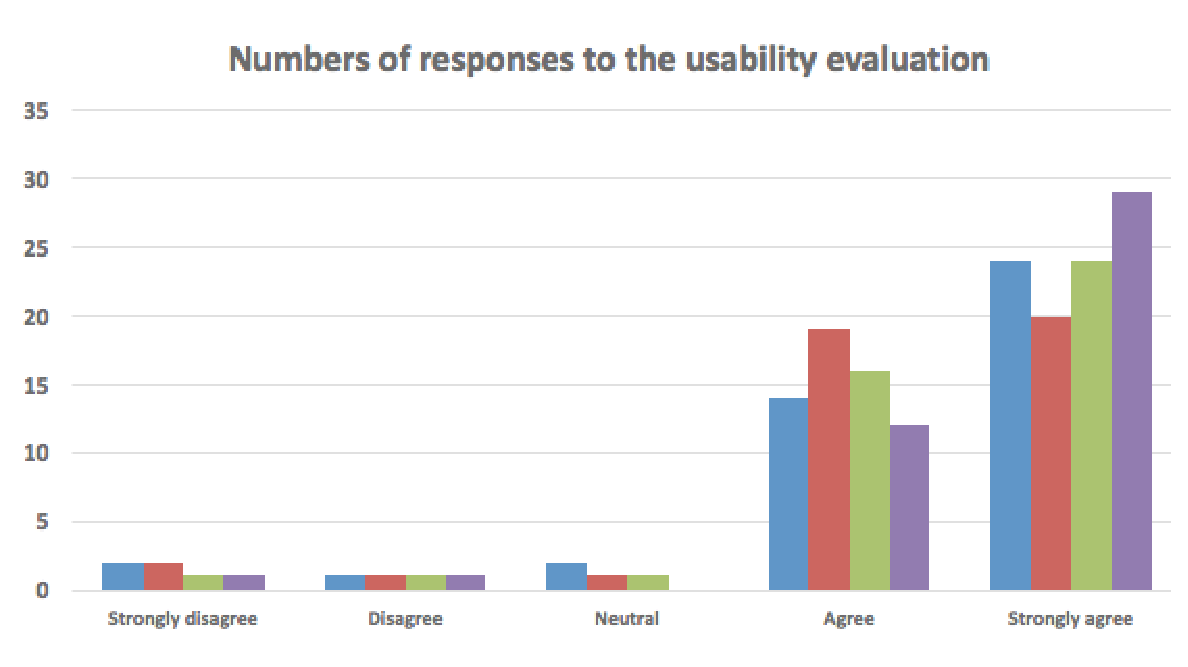
\includegraphics[height=3in]{self-report-usability-2011.eps}}
		\subfigure[2014 Self-reported Usability Measurements(n=18)]{\label{fig:self-report-usability-2014}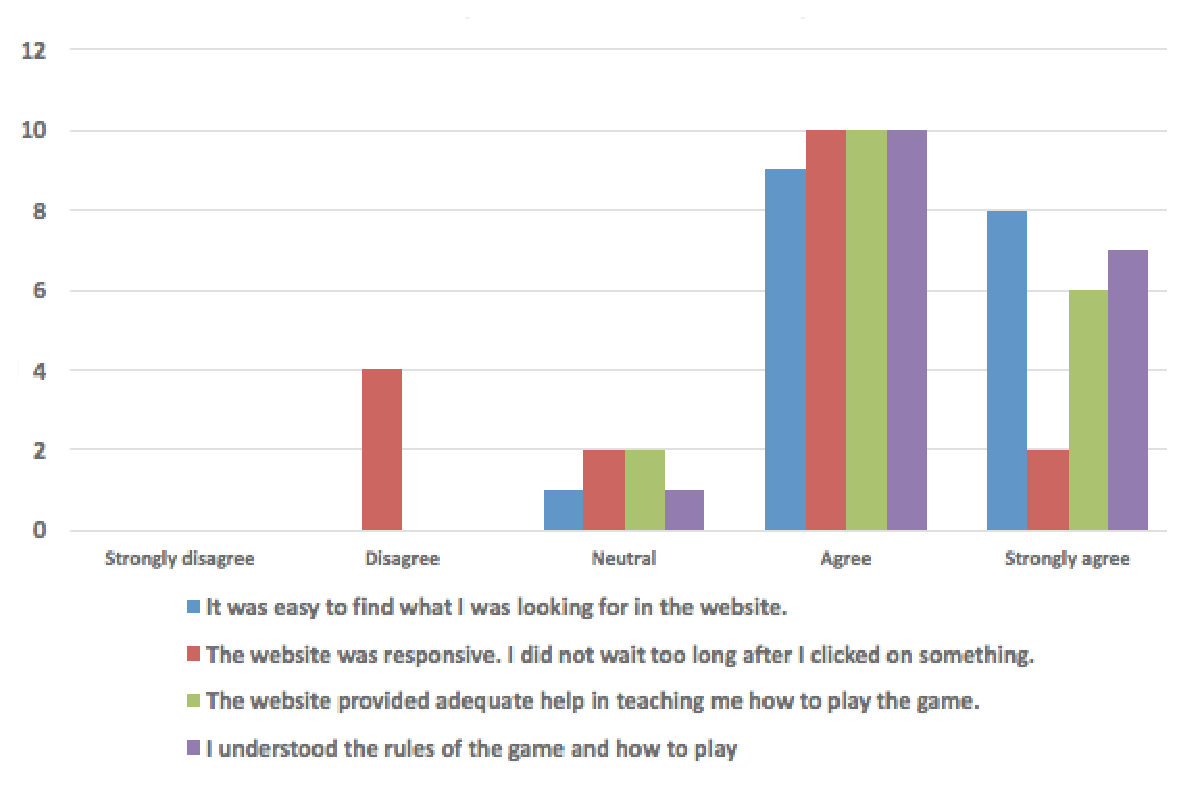
\includegraphics[height=3in]{self-report-usability-2014.eps}}
		\caption{Self-reported Usability Measurements in 2011 KC and 2014 KC}
		\label{fig:self-report-usability-2011-2014}
\end{figure}

Another question was asked in the 2014 UHM KC survey regarding the issues encountered when playing using the website. There are 3 out of 18 responses (17\%) reported that the loading of the website page were slow. This confirms the responsiveness issues discovered in the self-reported usability measurements described above. Another issues reported in the responses to the survey question is the confusion of the scoreboard display in the website. 3 out of 18 responses (17\%) reported that scoreboard's display keep changing so it is not easy to see their rankings. There are also 2 responses reported that some of the videos were not displayed which is due to the links to the videos were outdated.

In summary , the self-reported usability survey is a good tool to get feedback from the players of Makahiki to reveal the strengths and weaknesses regarding the usability of the game. 

\subsubsection{Engagement metrics}

Based on the engagement metrics \ref{Engagement metrics} proposed in the SGSEAM, we calculated a variety of engagement metrics to assess the player's engagement level in the Kukui Cup challenge created by the Makahiki framework. The metrics are calculated by analyzing the website logs and the data collected by the website. The results shown in \autoref{fig:makahiki-engagement} are the engagement metrics for the 2011 Kukui Cup challenge at the University of Hawaii at Manoa.
    
\begin{figure}[ht!]
  \centering
  \begin{tabular}{|l|c|c|c|c|c|c|}
    \hline
    \tabhead{\multirow{2}{*}{Measurement}} & \multicolumn{3}{c|}{\tabhead{2011 KC}} & \multicolumn{3}{c|}{\tabhead{2012 KC}}\\
     \cline{2-7}
    \tabhead{} & \tabhead{MIN} & \tabhead{AVG} & \tabhead{MAX} &  \tabhead{MIN} & \tabhead{AVG} & \tabhead{MAX}\\

    \hline
    Participation rate & 13\% & 37\% & 74\% & 19\% & 34\% & 64\%\\
    \hline
    Number of players per day & 43 & 85 & 147 & 0 & 12 & 130 \\
    \hline
    Play time per day & 1 min & 27.7 mins & 8.5 hours & 0 & 6.2 mins & 8.8 hours\\
    \hline
    Submissions per day & 32 & 266 & 1110 & 0 & 30 & 953\\
    \hline
    Social interactions per day & 51 &  208 & 468 & 0 & 31 & 502\\
    \hline
    Website errors per day & 0 & 0.6 & 4 & 0 & 2 & 458\\
    \hline
  \end{tabular}
  \caption{Engagement Metrics for 2011 and 2012 UHM Kukui Cup}
  \label{fig:makahiki-engagement}
\end{figure}

The participation rate is the percentage of players who played the game. The 2011 UHM KC had a 37\% average participation rate, while the 2012 KC had 34\%. Both are good compared to other sustainability challenges. 

Over the 3 weeks course of the challenge in the 2011 KC, an average player spent about 27.7 minutes per day on the website, while in the 24 weeks challenge in 2012 KC, an average player spent about 6.2 minutes per day. Both instances had one player spent over 8 hours (8.5 and 8.8 respectively) on one day, which is quite significant amount of time for a student to spent in this kind of game. The daily minimum time spent on the 2011 KC is 1 minute which indicates that for every day during the challenge, there are at least one player who played at least 1 minute. The daily minimum time spent on the 2012 KC is 0 minutes. This indicates that there are at least one day when no player use the website.

In order to investigate the engagement in a more details, we looked at the engagement measurement in a time series format. \autoref{fig:timeseries-metrics} shows the timed measurements graph during the 2011 and 2012 Kukui Cup.

\begin{figure}[ht!]
  \center
  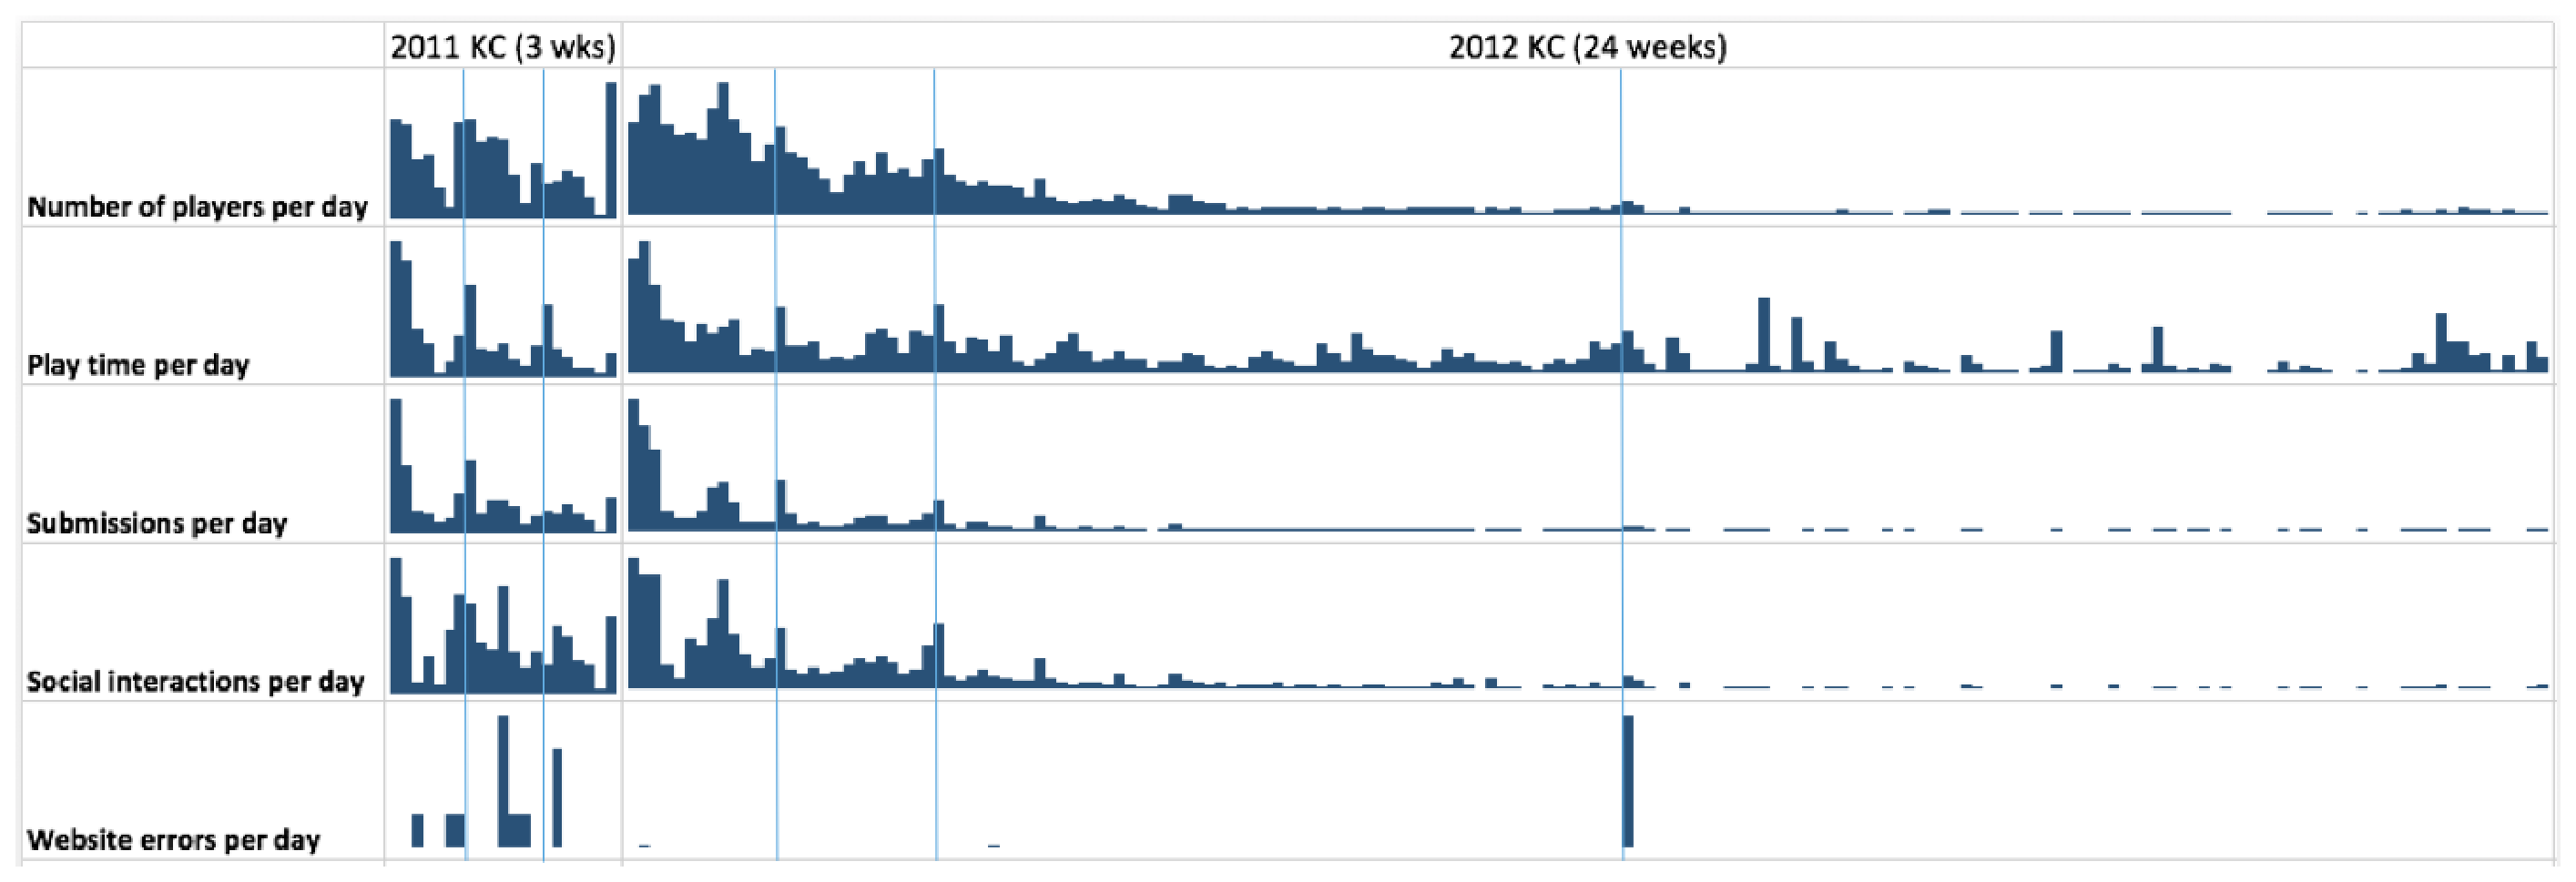
\includegraphics[height=3.2in,width=6.2in]{timeseries-metrics}
  \caption{Engagement Measurements during the 2011 and 2012 UHM Kukui Cup}
  \label{fig:timeseries-metrics}
\end{figure}

The divided line in the graphs indicates the division of the rounds for the 2011 and 2012 KC. In the 2011 KC, there are 3 rounds, each round lasted 1 week. In the 2012 KC, there are 4 rounds, the first and second round lasted 2 weeks each, and the third round lasted about 8 weeks, while the last round lasted about 12 weeks, with the total of 24 weeks for the 2012 KC. 

In addition to the daily number of players and daily play time which indicate the level of visits to the website or game, the daily submission and daily social interaction measurement indicate the level of deeper interactions with the game. We can see that during the 3 short weeks of the 2011 KC, the engagement patterns are similar in each week. The first few days has higher level of interactions then decreased later into the week. There is a spike on the last day of the round, which may be due to the urge of the players to check the winning results of the round. 

We can also see that in the 2012 KC, the engagement level significantly dropped after the second round, which is 4 weeks after the beginning of the game. There are still some numbers of players spent times on the game but the number of submissions and social interactions had decreased significantly. Over the time, the number of players decreased in the third round and even less in the last round. It is interesting to see that there are still some amounts of play time during the third and fourth round. A closer look at the data indicated that they are time spent from the the several top players who may be winning the game. 

Although the website error in the 2012 KC shown in the  \autoref{fig:makahiki-engagement} seems high, the detailed graph in \autoref{fig:timeseries-metrics} shows that the errors mostly happened during in one day which is the day after the start of the last round. The investigation of the error in the log file revealed that they are due to a content configuration error in a newly available event in the last round. The error caused the players not able to submit the completion of the event to claim their points so they kept trying and encountered the error repeatedly. The error was corrected 2 hours later after the first such error occurred.

In summary, SGSEAM indicates that Makahiki can be successful in achieving player engagement and literacy improvement. SGSEAM could not provide evidence of positive change in
behavior.

\subsection{Makahiki System Admin Assessment}
We used two approaches to assess the system administrators' experience with the Makahiki framework. They are in-lab installation study and post-hoc system admin interview.

\subsubsection{In-lab installation study}

In the in-lab installation study, the participants are the students in a serious game class (ICS691) in the Spring 2012 in the computer science department at the University of Hawaii at Manoa. The students were tasked with installing the Makahiki system into their local computers as well as deploying to the Heroku cloud environment. A Google Form was used to ask the students to record the time they spent completing each step and the problems they encountered. The students also provided feedback about their installation experiences in the form of blog posts. 

The results from the Google Form responses show that the average total time to successfully install
Makahiki was 1.4 hours, with a maximum time of 2 hours and the minimum time of 0.9 hour.
\autoref{fig:install-time} shows the average time for each installation step.

\begin{figure}[ht!]
  \center
  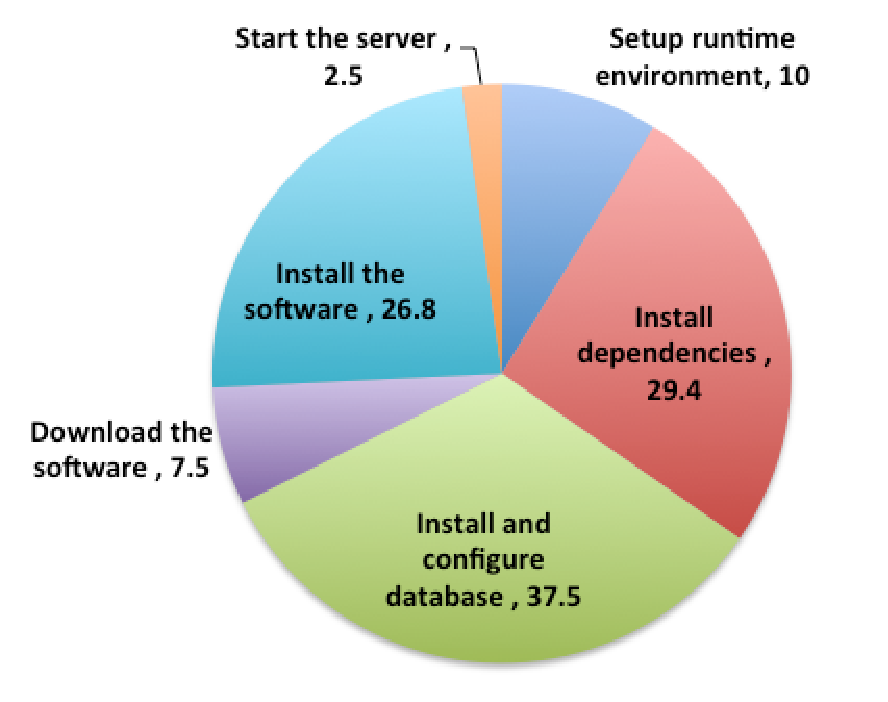
\includegraphics[width=0.7\columnwidth]{install-time}
  \caption{Average time (minutes) for installation steps (n=8)}
  \label{fig:install-time}
\end{figure}

We coded and categorized the descriptive problems reported by the students in both the Google Form
and their blog posts. \autoref{fig:makahiki-install} shows the result of the analysis from
the feedback of the 8 students that participated in the experiment.

\begin{figure}[ht!]
  \centering
  \begin{tabular}{|c|c|}
    \hline
    \multicolumn{1}{|p{0.7\columnwidth}|}{\centering\tabhead{Problem encountered}} &
    \multicolumn{1}{|p{0.2\columnwidth}|}{\centering\tabhead{Number of participants}} \\
    \hline
    \multicolumn{1}{|p{0.7\columnwidth}|}{Cannot find configuration file to edit during database installation } &
    \multicolumn{1}{|p{0.2\columnwidth}|}{4} \\
    \hline
    \multicolumn{1}{|p{0.7\columnwidth}|}{Documentation of install script is confusing about creation of the DB user} &
    \multicolumn{1}{|p{0.2\columnwidth}|}{2} \\
    \hline
    \multicolumn{1}{|p{0.7\columnwidth}|}{More parts of installation could be covered by install script} &
    \multicolumn{1}{|p{0.2\columnwidth}|}{2} \\
    \hline
  \end{tabular}
  \caption{Makahiki Installation Analysis (n=8)}
  \label{fig:makahiki-install}
\end{figure}


From the above analysis, we identified that the ``Install and configure database'' step has the
longest average time. It is also has the most participant reported problems. This reflects the issues
encountered by students during the configuration process. This assessment determines the areas for future
improvement are (1) to improve documentation on DB installation, and (2) to improve the install script to automate
more installation tasks.

In summary, SGSEAM identified database installation as a weak point in
installation.  Otherwise, SGSEAM indicates generally positive results regarding
Makahiki with respect to installation.

\subsubsection{Post-hoc System Admin Interview}
In order to gain insights on the experience of a real world system admin who uses the Makahiki, I performed interviews to the system admins of the Hawaii Pacific University (HPU) Kukui Cup challenges. The interview questions are outlined in the system admin assessment section of the SGSEAM. The interview took place after the challenge. Before the challenge, the system admin performed the installation of the Makahiki in the HPU local infrastructure. Issues encountered during the installation were communicated through emails and phone calls. They are recorded and analyzed as well as the interview data.

I analyzed qualitative data collected from the interviews and email changes. The data include: � time taken to install the Makahiki
� time taken to maintain the Makahiki, such as backup, monitoring
� problems encountered

\subsection{Makahiki Game Designer Assessment}

\subsubsection{In-lab game design study}

We also used the in-lab experiment to assess the game
designer experience of Makahiki. One of the class assignments for the students in the
experiment was to design a serious game using the Makahiki framework. We asked the students
to follow specific design steps and record the time required and any problems encountered during
their design process, using a Google Form similar to the one used for the system admin
assessment. In addition, students were asked to provide feedback about their
design experiences in the form of blog posts. \cite{csdl2-13-04} describes in detailed
the Google Form that is used in this assessment.

The game designer assessment was generalized into 7 tasks corresponding to
distinct types of administrative tasks and game design planning. The time for each task is
calculated from the Google Form results.  The most time consuming task
 is "Smart Grid Game Design", which took average 107.9 minutes (56\% of total time) to complete,
 while the least time
  consuming tasks is "Raffle Game Design", which took average 7.9 minutes (7\% of total time)
  to complete.

\autoref{fig:design-time} shows the average time for each design tasks:

\begin{figure}[ht!]
  \center
  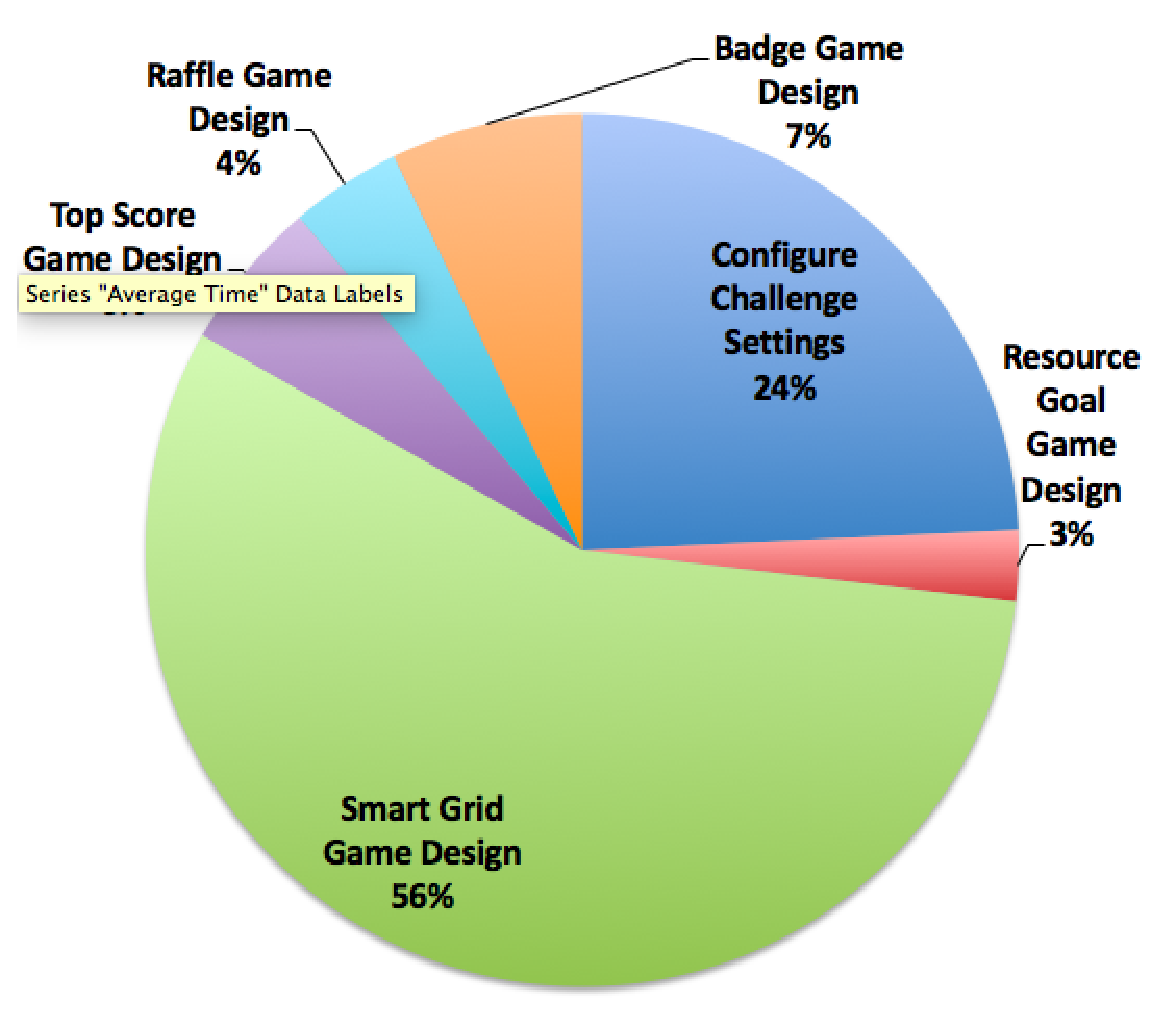
\includegraphics[width=0.7\columnwidth]{design-time}
  \caption{Average time (minutes) for design tasks (n=8)}
  \label{fig:design-time}
\end{figure}

 We aggregated the problems reported in the feedback of the 7 students that participated in the experiment.
\autoref{fig:makahiki-game-design} shows the result of the analysis:

\begin{figure}[ht!]
  \centering
  \begin{tabular}{|c|c|c|}
    \hline
    \multicolumn{1}{|p{0.7\columnwidth}|}{\centering\tabhead{Problem encountered}} &
    \multicolumn{1}{|p{0.2\columnwidth}|}{\centering\tabhead{Number of participants}} \\
    \hline
    \multicolumn{1}{|p{0.7\columnwidth}|}{Difficulty in understanding predicate system and unlock condition} &
    \multicolumn{1}{|p{0.2\columnwidth}|}{7} \\
    \hline
    \multicolumn{1}{|p{0.7\columnwidth}|}{A bug that prevented users with usernames
containing capital letters from logging in} &
    \multicolumn{1}{|p{0.2\columnwidth}|}{2} \\
    \hline
    \multicolumn{1}{|p{0.7\columnwidth}|}{A bug in the processing of Ajax queries} &
    \multicolumn{1}{|p{0.2\columnwidth}|}{1} \\
    \hline
    \multicolumn{1}{|p{0.7\columnwidth}|}{Difficulty in generating event attendance codes for game activities} &
    \multicolumn{1}{|p{0.2\columnwidth}|}{1} \\
    \hline
  \end{tabular}
  \caption{Makahiki Game Design Analysis, (n=8)}
  \label{fig:makahiki-game-design}
\end{figure}

In summary, SGSEAM revealed two shortcomings with Makahiki configuration: ``Smart
Grid Game Design'' and ``Configure Challenge Settings''. Issues encountered in ``Smart Grid Game
Design'' included 1) difficulty and lack of documentation on the predicate system used to define dependencies
between game activities, and 2) difficulty in generating event attendance codes for game activities.
Issues encountered in ``Configure Challenge Settings'' included 1) a bug in the processing of Ajax queries
caused by consecutive clicks on the same interface button, and 2) a bug that prevented users with username
containing capital letters from logging in.

\subsection{Makahiki Game Manager Assessment}
We used the 2012 Kukui Cup Challenge at the Hawaii Pacific University (HPU) to assess
the game manager experience of Makahiki. We interviewed the
game manager of the HPU Kukui Cup challenge, who is also the game designer of the challenge.
We asked him about his game management experiences using the Makahiki admin
interface. The interview questions are outlined in the game manager section of the SGSEAM.

The interview took place after the challenge and was audio-recorded. We transcribed the
audio recording. The data shows that the game management interface was easy for him to use.
He made sure that player submissions were either approved or rejected
within 12 hours. He also discovered a useful feature in the approval interface without
help from the Makahiki support team. The only problem he reported was that after the
competition ended, he discovered that some of the analytics data disappeared. This was
identified by the Makahiki development team as a software bug and has since been fixed.

In summary, SGSEAM uncovered few problems with Makahiki game management using the interview
approach. We realized that the confident level of this assessment approach is low because of
 availability of only one data point. An experimental study approach or perform interviews to
multiple game managers will increase the confidence level of the assessment.

\subsection{Makahiki Developer Assessment}

We assessed developer experience using an in-lab experiment. One of the class assignments
for the students in the experiment was to develop an enhancement to Makahiki.  This
involved setting up a development environment, following the tutorial to create a ``Hello
world'' widget using Makahiki, and finally, developing an enhancement to extend the
functionality of Makahiki.

The students were asked to submit their development source code to the
public source code repository (GitHub) and write a blog post to
discuss their efforts to complete the development activity.

All 8 students reported that the first task of creating the simple ``Hello world'' widget
was easy, while the enhancement development was hard. Only one student successfully
completed all 5 required features, while the rest successfully completed 1 or 2
features. The main problem students reported was the lack of documentation for the
development libraries. One student stated in his blog that he decided to choose Makahiki
framework to develop his own serious game because of Makahiki's features and possibility
of reducing development effort by using the framework.

In summary, SGSEAM reveals significant problems with developer efficiency.
Analysis is still ongoing regarding the specific causes of problems and how best to
address them.
